\documentclass[cn,11pt,chinese,black,simple]{elegantbook}

\def\mainclass{main}

\title{信号与系统}
% \subtitle{数字设计初步}

\author{Pannenets.F}
% \institute{微电子学院}
\date{\today}
% \version{4}
\bioinfo{分类}{笔记}

\extrainfo{Je reviendrai et je serai des millions. —— <<Spartacus>>}
% \logo{logo-blue.png}
\cover{logo.png}

% 本文档命令
\usepackage{array}
\newcommand{\ccr}[1]{\makecell{{\color{#1}\rule{1cm}{1cm}}}}


\newcommand{\where}[1]{\Big|_{#1}}
\newcommand{\dd}[1]{\mathrm{d}#1}
\newcommand{\abs}[1]{\left| #1 \right|}
\newcommand{\zt}[1]{\mathscr{Z}[#1]}
\newcommand{\zta}{\xrightarrow{\mathscr{Z}}} 
\newcommand{\lt}[1]{\mathscr{L}[#1]}
\newcommand{\lta}{\xrightarrow{\mathscr{L}}} 
\newcommand{\ft}[1]{\mathscr{F}[#1]}
\newcommand{\fta}{\xrightarrow{\mathscr{F}}} 
\newcommand{\dsum}{\displaystyle\sum}
\newcommand{\aint}{\int_{-\infty}^{+\infty} }

\newcommand{\re}{\operatorname{Re}[\mathrm{s}]} 


\newcommand{\qfig}[2]{\begin{figure}[!htb]
  \centering
  \includegraphics[width=0.6\textwidth]{#1}
  \caption{#2}
\end{figure}}



\renewcommand\arraystretch{1.6}




\setcounter{tocdepth}{3}
\newcommand{\dollar}{\mbox{\textdollar}}
\lstset{
  mathescape = false}

  

\usepackage{shapepar}
\usepackage{longtable}
\usepackage{tikz}
% \usepackage{multirow}
\usetikzlibrary{positioning}
\tikzset{>=stealth}
\newcommand{\tikzmark}[3][]
  {\tikz[remember picture, baseline]
    \node [anchor=base,#1](#2) {#3};}
\usetikzlibrary{graphs}


\begin{document}

\maketitle
% \frontmatter

% \chapter*{特别声明}
% \markboth{Introduction}{前言}

% 本书用于个人\textbf{信号与系统 2020 春}课程的复习,对课本中一些错误进行了修订,但是作者不对可能出现的笔误等负责。欢迎指正。


% \vskip 1.5cm


% \begin{flushright}
% Pannenets.F \\
% \today
% \end{flushright}

\tableofcontents
\listoffigures
\listoftables
%\listofchanges

\mainmatter


% TODO: 常微分方程配凑形式
% DONE: 差分方程配凑形式 

\ifx\mainclass\undefined
\documentclass[cn,11pt,chinese,black,simple]{../elegantbook}
\usepackage{array}
\newcommand{\ccr}[1]{\makecell{{\color{#1}\rule{1cm}{1cm}}}}


\newcommand{\where}[1]{\Big|_{#1}}
\newcommand{\dd}[1]{\mathrm{d}#1}
\newcommand{\abs}[1]{\left| #1 \right|}
\newcommand{\zt}[1]{\mathscr{Z}[#1]}
\newcommand{\zta}{\xrightarrow{\mathscr{Z}}} 
\newcommand{\lt}[1]{\mathscr{L}[#1]}
\newcommand{\lta}{\xrightarrow{\mathscr{L}}} 
\newcommand{\ft}[1]{\mathscr{F}[#1]}
\newcommand{\fta}{\xrightarrow{\mathscr{F}}} 
\newcommand{\dsum}{\displaystyle\sum}
\newcommand{\aint}{\int_{-\infty}^{+\infty} }

\newcommand{\re}{\operatorname{Re}[\mathrm{s}]} 


\newcommand{\qfig}[2]{\begin{figure}[!htb]
  \centering
  \includegraphics[width=0.6\textwidth]{#1}
  \caption{#2}
\end{figure}}



\renewcommand\arraystretch{1.6}




\setcounter{tocdepth}{3}
\newcommand{\dollar}{\mbox{\textdollar}}
\lstset{
  mathescape = false}

  

\usepackage{shapepar}
\usepackage{longtable}
\usepackage{tikz}
% \usepackage{multirow}
\usetikzlibrary{positioning}
\tikzset{>=stealth}
\newcommand{\tikzmark}[3][]
  {\tikz[remember picture, baseline]
    \node [anchor=base,#1](#2) {#3};}
\usetikzlibrary{graphs}
\begin{document}
\fi 

% Start Here

\chapter{信号与系统概论}



本章讨论信号与系统的基础概念问题。

\section{信号的分类}

\begin{definition}[能量/功率信号]\label{def:ene-powersig}
  对于信号 \(f(t)\) , 定义其能量为 : 
  \[W = \lim_{T\rightarrow \infty} \int_{-T/2}^{T/2} f^2(t) \dd{t} \]
  定义其功率为 : 
  \[P = \lim_{T\rightarrow \infty} \dfrac{1}{T} \int_{-T/2}^{T/2} f^2(t) \dd{t} \] 
\end{definition}

\section{信号的变换}

掌握信号的压缩、扩展、反褶以及时移等运算。

\section{基本信号}

本书涉及到的基本信号可以列举如下。

\begin{itemize}
  \item 指数类信号 
    \begin{itemize}
      \item 实指数信号 \(K e^{\alpha t}\)
      \item 复指数信号 \(K e^{(\sigma + j \omega)t}\)
      \item 正余弦信号 \(\cos(\omega t + \varphi)\), \(\sin(\omega t + \varphi)\)
    \end{itemize}
  \item 奇异信号
    \begin{itemize}
      \item 单位冲激信号 \(\delta(t)\)
      \item 单位阶跃信号 \(u(t)\)
      \item 单位斜变信号 \(r(t)\)
    \end{itemize}
\end{itemize}

\section{系统的描述}

本课程研究的系统均可用微分方程或者差分方程描述,这样的系统可以使用框图进行描述。

系统可以使用以下标准进行分类。

\begin{itemize}
  \item 连续时间系统与离散时间系统
  \item 有记忆系统与无记忆系统
  \item 可逆系统与不可逆系统 : 不同的激励是否会引起不同的相应
  \item 因果系统与非因果系统 : 响应出现不早于激励
  \item 稳定系统与不稳定系统 : 有限输入是否引起有限输出
  \item 线性系统与非线性系统
  \item 时变系统与时不变系统 : 输入的时移对应引起输出的时移
\end{itemize}



% End Here

\ifx\mainclass\undefined
\end{document}
\fi 

\ifx\mainclass\undefined
\documentclass[cn,11pt,chinese,black,simple]{../elegantbook}
\usepackage{array}
\newcommand{\ccr}[1]{\makecell{{\color{#1}\rule{1cm}{1cm}}}}


\newcommand{\where}[1]{\Big|_{#1}}
\newcommand{\dd}[1]{\mathrm{d}#1}
\newcommand{\abs}[1]{\left| #1 \right|}
\newcommand{\zt}[1]{\mathscr{Z}[#1]}
\newcommand{\zta}{\xrightarrow{\mathscr{Z}}} 
\newcommand{\lt}[1]{\mathscr{L}[#1]}
\newcommand{\lta}{\xrightarrow{\mathscr{L}}} 
\newcommand{\ft}[1]{\mathscr{F}[#1]}
\newcommand{\fta}{\xrightarrow{\mathscr{F}}} 
\newcommand{\dsum}{\displaystyle\sum}
\newcommand{\aint}{\int_{-\infty}^{+\infty} }

\newcommand{\re}{\operatorname{Re}[\mathrm{s}]} 


\newcommand{\qfig}[2]{\begin{figure}[!htb]
  \centering
  \includegraphics[width=0.6\textwidth]{#1}
  \caption{#2}
\end{figure}}



\renewcommand\arraystretch{1.6}




\setcounter{tocdepth}{3}
\newcommand{\dollar}{\mbox{\textdollar}}
\lstset{
  mathescape = false}

  

\usepackage{shapepar}
\usepackage{longtable}
\usepackage{tikz}
% \usepackage{multirow}
\usetikzlibrary{positioning}
\tikzset{>=stealth}
\newcommand{\tikzmark}[3][]
  {\tikz[remember picture, baseline]
    \node [anchor=base,#1](#2) {#3};}
\usetikzlibrary{graphs}
\begin{document}
\fi 

% Start Here

\chapter{连续时间系统的时域分析}

\section{常系数线性微分方程}

常微分方程的求解可以分为以下几个步骤。

\begin{enumerate}
  \item 根据特征方程求解齐次解
  \item 根据激励形式配凑特解,求得对应的系数
  \item 将完全解代入系统初始条件,确定待定系数
\end{enumerate}



\begin{longtable}{ll} 
  \caption{微分方程特解的形式} \\ 
  \toprule
  激励 &  特解形式\\
  \midrule
  \endfirsthead
  
  \toprule
  激励 &  特解形式\\
  \midrule
  \endhead 

  \hline
  \multicolumn{2}{c}{见下页}\\   \bottomrule
  \endfoot

  \bottomrule
  \endlastfoot

  常数\(E\) & 常数\(D\) \\
  \(t^n\) & \(A_1 t^n + A_2 t^{n-1} + \cdots + A_n t + A_{n+1}\) \\
  \(e^{\alpha t}\) & \(A e^{\alpha t}\) \\
  \(\cos (\beta n)\) 或 \(\sin (\beta n)\) & \(P \cos(\beta n) + Q \sin(\beta n)\) \\
  \(t^n e^{\alpha t}\cos (\beta n)\) 或 \(t^n e^{\alpha t}\sin (\beta n)\) & \begin{tabular}[c]{@{}l@{}}\((A_1 t^n + A_2 t^{n-1} + \cdots + A_n t + A_{n+1})e^{\alpha t} \cos(\beta n) +\)\\ \( (B_1 t^n + B_2 t^{n-1} + \cdots + B_n t + B_{n+1})e^{\alpha t}\)\end{tabular} \\

\end{longtable}

\section{常微分方程解的分类}

解的分类。

\begin{itemize}
  \item 自由响应:齐次解
  \item 强迫响应:特解
  \item 暂态响应:时间趋于无穷时解中趋于 0 的部分
  \item 稳态响应:时间趋于无穷时解中不为 0 的部分
  \item 零输入响应:完全由系统储能引起的响应
  \item 零状态响应:完全由激励引起的响应
\end{itemize}



系统时间点的区分。

\begin{itemize}
  \item 起始状态: \(t = 0_-\)
  \item 初始状态: \(t = 0_+\)
\end{itemize}

\section{单位冲激响应}

对于微分方程的单位冲激响应的一般求法,给定一般的系统方程:

\[
\dsum_{i=0}^{n} C_i \dfrac{\dd{^{n-i} r(t)}}{\dd{t^{n-i}}} = \dsum_{j=0}^{m} E_j \dfrac{\dd{^{m-j} e(t)}}{\dd{t^{m-j}}} 
\]

\begin{enumerate}
  \item 将 \(C_0\) 化为 \(1\) ,并且将激励的一侧使用冲激函数 \(\delta(t)\) 完全代替
  \item 为了满足冲激函数的匹配性,那么只有右侧最高阶导数 \(\dfrac{\dd{^n r(t)}}{\dd{t^n}}\) 中含有 \(\delta(t)\)
  \item 那么有\(\dfrac{\dd{^{n-1} r(t)}}{\dd{t^{n-1}}}\left|_{t=0^+}\right. = 1\) 以及 \(\dfrac{\dd{^{i} r(t)}}{\dd{t^{i}}}\left|_{t=0^+}\right. = 0, i < (n-1)\)
  \item 之后根据线性性以及时不变性得到单位冲激响应
\end{enumerate}

\section{卷积计算及性质}

\begin{definition}[卷积]
  对于函数 \(x(t)\), \(y(t)\) 定义其卷积为
  \[s(t) = \int_{-\infty}^{+\infty} x(\tau) y(t-\tau) \dd{\tau}\]
  通常可以表示为
  \[s(t) = x(t) \otimes y(t)\]
  或者
  \[s(t) = x(t) * y(t))\]
\end{definition}

卷积的性质。
\begin{itemize}
  \item 分配率
  \item 交换律
  \item 结合律
  \item 微分积分性质 \[s^{(n-m)}(t) = f_1^{(n)}(t) \otimes f_2^{(-m)}(t) = f_1(t) \otimes f_2'(t)\]
  \item 冲激函数性质 \[f(t-t_1) \otimes \delta(t-t_0) = f(t-t_0-t_1)\] 
        \[f(t) \otimes \delta'(t) = f'(t)\] 
        \[f(t) \otimes \delta^{-1}(t) = \int_{-\infty}^t f(\tau)\dd{\tau}\]
\end{itemize}

\section{时域系统的特性}

LTI 系统的系统性质围绕着单位冲激响应展开。

因果性的\textbf{充要条件}: \[h(t) = h(t) u(t)\]

稳定性的\textbf{充要条件}(绝对可积): \[\int_{-\infty}^{+\infty} |h(t-\tau)| \dd{\tau} \leq N \] 


% End Here

\ifx\mainclass\undefined
\end{document}
\fi 

\ifx\mainclass\undefined
\documentclass[cn,11pt,chinese,black,simple]{../elegantbook}
\usepackage{array}
\newcommand{\ccr}[1]{\makecell{{\color{#1}\rule{1cm}{1cm}}}}


\newcommand{\where}[1]{\Big|_{#1}}
\newcommand{\dd}[1]{\mathrm{d}#1}
\newcommand{\abs}[1]{\left| #1 \right|}
\newcommand{\zt}[1]{\mathscr{Z}[#1]}
\newcommand{\zta}{\xrightarrow{\mathscr{Z}}} 
\newcommand{\lt}[1]{\mathscr{L}[#1]}
\newcommand{\lta}{\xrightarrow{\mathscr{L}}} 
\newcommand{\ft}[1]{\mathscr{F}[#1]}
\newcommand{\fta}{\xrightarrow{\mathscr{F}}} 
\newcommand{\dsum}{\displaystyle\sum}
\newcommand{\aint}{\int_{-\infty}^{+\infty} }

\newcommand{\re}{\operatorname{Re}[\mathrm{s}]} 


\newcommand{\qfig}[2]{\begin{figure}[!htb]
  \centering
  \includegraphics[width=0.6\textwidth]{#1}
  \caption{#2}
\end{figure}}



\renewcommand\arraystretch{1.6}




\setcounter{tocdepth}{3}
\newcommand{\dollar}{\mbox{\textdollar}}
\lstset{
  mathescape = false}

  

\usepackage{shapepar}
\usepackage{longtable}
\usepackage{tikz}
% \usepackage{multirow}
\usetikzlibrary{positioning}
\tikzset{>=stealth}
\newcommand{\tikzmark}[3][]
  {\tikz[remember picture, baseline]
    \node [anchor=base,#1](#2) {#3};}
\usetikzlibrary{graphs}
\begin{document}

\fi 



% Start Here
\chapter{连续时间信号的实频域分析}

本章在时域对信号进行分解进行研究,主要工具是傅里叶级数、傅里叶变换。这一章最重要的是掌握傅里叶变换的性质,进而大大简化计算过程。

\section{相关系数以及正交函数}

\begin{definition}[相关系数]
  记误差函数\(e(t)\)为\[e(t) = f(t) - k g(t)\]
  其均方误差为\[\bar{e^2(t)} = \int_{t_1}^{t_2}[f(t)-k g(t)]^2 \dd{t}\]
  在均方误差取得最小值时的 \(k\) 取值即为 \(f(t)\), \(g(t)\) 的相关系数,表征两者的相似程度
  \[k = \dfrac{\int_{t_1}^{t_2} f(t) g(t) \dd{t}}{\int_{t_1}^{t_2} g^2(t) \dd{t}}\]
\end{definition}

当两个函数的相关系数为 \(0\) 时,称这两个函数正交。

信号自身的正交分解常见两种:

\begin{itemize}
  \item 直流-交流分解 
  \item 奇偶分量分解
\end{itemize}

\section{三角函数形式傅里叶级数}

三角函数形式的傅里叶级数:

\[f(t) = a_0 + \dsum_{n=1}^{\infty} (a_n \cos n\omega_1 t + b_0 \sin \omega_1 t)\]

其中
\[a_0 = \dfrac{1}{T_1} \int_{-T_1/2}^{T/2} f(t) \dd{t}\]
\[a_n = \dfrac{2}{T_1} \int_{-T_1/2}^{T/2} f(t) \cos n \omega_1 \dd{t}\]
\[b_n = \dfrac{2}{T_1} \int_{-T_1/2}^{T/2} f(t) \sin n \omega_1 \dd{t}\]

三角函数形式的频谱分为幅度谱以及相位谱。幅度谱为
\[c_n = \sqrt{a_n^2 + b_n^2}\]

相位谱为
\[\phi_n = \tan^{-1}\left(\dfrac{-b_n}{a_n}\right)\]

\section{指数函数形式傅里叶级数}

指数形式的傅里叶级数:

\[f(t) = \dsum_{n=-\infty}^{+\infty} F(n\omega_1) e^{j n \omega_1 t}\]

其中
\[F(n\omega_1) = \dfrac{1}{T_1} \int_{-T_1/2}^{T_1/2} f(t) e^{-j n \omega_1 t} \dd{t}\]

根据三角函数形式级数的运算可以得到

\[a_{-n} = a_n, b_{-n} = -b_n\]

那么有

\[F(n \omega_1) = \left\{
\begin{aligned}
  & a_0, \text{n = 0}\\
  & \dfrac{a_n - j b_n}{2}, \text{n \(\neq\) 0}
\end{aligned}\right.
\]

称\(F{n\omega_1}\)为信号的复数频谱或者复数谱。

类似的,频谱为
\[ F(n \omega_1) = |F(n \omega_1)| e^{j \varphi_n} \]

\section{三角函数-指数函数形式傅里叶级数的频谱关系}

三角函数幅度谱与相位谱均为单边谱,对于幅度谱为偶拓延

\[ 
|F(n \omega_1)| = \left\{\begin{aligned}
  c_0 = a_0, n = 0 \\
  \dfrac{1}{2} \sqrt{a_n^2 + b_n^2} = \dfrac{1}{2} c_n , n \neq 0
\end{aligned}\right\}
\]

对于相位谱为奇拓延

\[
\varphi_n = \arctan (\dfrac{-b_n}{a_n})  
\]

\section{对称性}

\begin{longtable}{lll} 
  \caption{傅里叶级数的奇偶对称性} \\ 
  \toprule
  函数分类 & 三角级数性质 & 指数级数性质\\ 
  \midrule
  \endfirsthead
  
  \toprule
  函数分类 & 三角级数性质 & 指数级数性质\\ 
  \midrule
  \endhead 

  \hline
  \multicolumn{3}{c}{见下页}\\   \bottomrule
  \endfoot

  \bottomrule
  \endlastfoot
  奇函数                                                                              & 只包含正弦函数分量                                                      & \(F(n \omega_1)\) 为纯虚数 相位谱只取\(\pm \dfrac{1}{2} \pi\) \\ 
  偶函数                                                                              & 只包含余弦函数分量                                                      & \(F(n \omega_1)\) 为实数 相位谱只取\(\pm  \pi\)             \\ 
  \begin{tabular}[c]{@{}l@{}}奇谐函数\footnote{定义为\(f(t) = -f(t\pm \dfrac{T}{2})\)}\\\end{tabular} & \begin{tabular}[c]{@{}l@{}}只含有奇次谐波,\\ 不含偶次谐波与直流分量\end{tabular} &                                                     \\
  \begin{tabular}[c]{@{}l@{}}偶谐函数\footnote{定义为\(f(t) = f(t\pm \dfrac{T}{2})\)}\\\end{tabular}  & \begin{tabular}[c]{@{}l@{}}只含有次谐波与直流分量,\\ 不含有奇次谐波\end{tabular} &                    

\end{longtable}

\section{傅里叶变换}

\begin{definition}[傅里叶变换]
  对于任意的函数\(f(t)\),将其频谱密度函数
  \[F(\omega) = \int_{-\infty}^{+\infty} f(t) e^(-j\omega t) \dd{t}\]
  定义为傅里叶变换
\end{definition}
\section{傅里叶变换的性质}

假定已知变换为

\[f(t) \fta F(\omega)\]

性质列表如下


\begin{longtable}{ll} 
  \caption{傅里叶变换性质} \\ 
  \toprule
  名称 & 表达形式 \\ 
  \midrule
  \endfirsthead
  
  \toprule
  名称 & 表达形式 \\ 
  \midrule
  \endhead 

  \hline
  \multicolumn{2}{c}{见下页}\\   \bottomrule
  \endfoot

  \bottomrule
  \endlastfoot

  对称性 & \( F(t) \fta 2 \pi f(-\omega) \) \\
  奇偶虚实性 & 同傅里叶级数 \\
  反褶性质 & \(f(-t) \fta F(-\omega) = F^*(\omega)\) \\
  时移性质 & \(f(t-t_0) \fta F(\omega) e^{-j \omega t_0}\) \\
  压扩性质 & \(f(at) \fta \dfrac{1}{|a|}F(\dfrac{\omega}{a})\) \\
  线性性 &  \\
  时域微分 & \(f'(t) \fta j\omega F(\omega)\) \\
   & \(f^{(n)}(t) \fta (j\omega)^{(n)} F(\omega)\) \\
  时域积分 & \(\int_{-\infty}^{t}f(\tau) \dd{\tau} \fta \dfrac{F(\omega)}{j\omega} + \pi F(0) \delta(\omega)\) \\
  频移特性 & \(f(t)e^{j \omega_0 t} \fta F(\omega - \omega_0)\) \\
  卷积定理 & \(f_1(t) \otimes f_2(t) \fta F_1(\omega)F_2(\omega)\)\\
  & \(f_(t)f_1(t) \fta \dfrac{1}{2\pi} F_1(\omega)\otimes F_2(\omega)\)
  
  
\end{longtable}

\section{周期信号的傅里叶变换}

对于周期为 \(T\) 的信号 \(f(t)\) 有傅里叶级数


\[f(t) = \dsum_{n=-\infty}^{+\infty} F(n\omega_1) e^{j n \omega_1 t}\]

其中
\[F(n\omega_1) = \dfrac{1}{T_1} \int_{-T_1/2}^{T_1/2} f(t) e^{-j n \omega_1 t} \dd{t}\]

对其单周期信号 \(f_1(t)\) 有

\[f_1(t) = f(t) \left[u(t+\dfrac{T_1}{2}) - u(t-\dfrac{T_1}{2})\right]\]

其傅里叶变换 \(F_1(\omega)\) 与原函数的傅里叶级数满足

\[F(n \omega_1) = \dfrac{1}{T_1}F_1(\omega)\left|_{\omega = n \omega_1}\right.\]

带入傅里叶级数中得到

\[f(t) \fta 2\pi \dsum_{-\infty}^{+\infty} F(n\omega_1) \delta(\omega - n\omega_1)\]

或者可以简单地通过卷积表示。单个周期信号为 \(f_0(t)\) 那么

\[f_{T_1}(t) = f_0(t) \otimes \delta_{T_1}(t)\]

\[\ft{f_{T_1}(t)} = F_0(\omega) \dfrac{1}{T_1}\dsum_{-\infty}^{\infty} 2\pi \delta(\omega - n\omega_1) = F_0(\omega) \omega_1 \dsum_{-\infty}^{\infty} \delta(\omega - n\omega_1) \] 


\section{常见信号的傅里叶变换对}

\begin{definition}[$Sa$ 函数]
\[Sa(t) = \dfrac{\sin t}{t}\]
\end{definition}

在数字信号处理和通信理论中,归一化 \(sinc(x)\) 函数通常定义为 \(Sa(\pi x)\) 。

\begin{longtable}{ll} 
  \caption{傅里叶变换对} \\ 
  \toprule
  时域信号 & 频域信号 \\ 
  \midrule
  \endfirsthead
  
  \toprule
  时域信号 & 频域信号 \\ 
  \midrule
  \endhead 

  \hline
  \multicolumn{2}{c}{见下页}\\   \bottomrule
  \endfoot

  \bottomrule
  \endlastfoot

  \(G_{\tau}(t) = u(t+\dfrac{\tau}{2}) - u(t - \dfrac{\tau}{2})\) & \(\tau Sa(\dfrac{\omega \tau}{2})\) \\ 
  \(G_{\tau}(t) \otimes G_{\tau}(t) = \left\{\begin{aligned}
      \tau - |t|, |t| < \tau \\
      0, t \geq \tau
  \end{aligned}\right. \) & \(\tau^2 Sa^2(\dfrac{\omega \tau}{2})\) \\
  \(e^{-\alpha t}u(t)\) & \(\dfrac{1}{\alpha + j \omega}\) \\
  \(e^{-\alpha |t|}\) & \(\dfrac{2\alpha}{\alpha ^2 + \omega^2}\) \\
  \(sgn(t)\) & \(\dfrac{2}{j \omega}\) \\
  \(\delta(t)\) & \(1\) \\
  \(1\) & \(2 \pi \delta(\omega)\) \\
  \(u(t)\) & \(\pi \delta(\omega) + \dfrac{1}{j \omega}\) \\
  \(\sin \omega_1 t\) & \(-j \pi[\delta(\omega-\omega_1) -\delta(\omega + \omega_1)]\) \\
  \(\cos \omega_1 t\) & \(\pi [\delta(\omega-\omega_1) + \delta(\omega+\omega_1)]\) \\
  \(\delta_{T_1}(t) = \dsum_{-\infty}^{\infty}\delta(t-nT_1) \) & \(\omega_1 \dsum_{-\infty}^{\infty} \delta(\omega - n \omega_1)\) \\
  \(G_{T_1,\tau}(t)\) & \(2\pi \dsum_{-\infty}^{\infty} \dfrac{\tau}{T_1} Sa(\dfrac{n \omega_1 \tau}{2} ) \delta(\omega - n\omega_1)\) \\
  
  
\end{longtable}

\section{抽样信号}

原始信号为 \(f(t)\) ,抽样脉冲信号为 \(p(t)\) 

\[f_s(t) = f(t) p(t)\]

抽样信号为周期信号 

\[p(t) \fta P(\omega) = \omega_s \dsum_{-\infty}^{\infty}P_0(n \omega_s) \delta(\omega - n\omega_s)\]

那么
\[f_s(t) \fta F_s(\omega) = \dfrac{1}{2\pi}F(\omega) \otimes \left[\omega_s \dsum_{-\infty}^{\infty}P_0(n \omega_s) \delta(\omega-n\omega_s)\right]\]

化简

\[f_s(t) \fta F_s(\omega) = \dfrac{1}{T_s} \left[ \dsum_{-\infty}^{\infty}P_0(n \omega_s) F(\omega-n\omega_s)\right]\]

\begin{theorem}[时域抽样定理]
  对于原始信号 \(f(t) \fta F(\omega)\) 以及抽样脉冲 \(p(t) \fta P(\omega)\) ,且原始信号带宽有限 \(\abs{\omega} < \omega_m\),
  可以得到抽样频谱 
  \[f_s(t) = p(t) f(t) \fta \dfrac{1}{2 \pi} F(\omega) \otimes P(\omega)\]

  为可以从抽样信号中恢复被抽样信号,在采样间隔 \(\omega_s\) 间,不能发生原信号的重叠,
  即
  \[\omega_s \geq 2 \omega_m\]
  或者可以化为 
  \[\dfrac{2\pi}{T_s} \geq 2 \times 2  \pi f_m\]
  \[T_s \leq \dfrac{1}{2 f_m}\]

  最小的采样频率称为奈奎斯特频率。
\end{theorem}



% End Here

\ifx\mainclass\undefined
\end{document}
\fi 

\ifx\mainclass\undefined
\documentclass[cn,11pt,chinese,black,simple]{../elegantbook}
\usepackage{array}
\newcommand{\ccr}[1]{\makecell{{\color{#1}\rule{1cm}{1cm}}}}


\newcommand{\where}[1]{\Big|_{#1}}
\newcommand{\dd}[1]{\mathrm{d}#1}
\newcommand{\abs}[1]{\left| #1 \right|}
\newcommand{\zt}[1]{\mathscr{Z}[#1]}
\newcommand{\zta}{\xrightarrow{\mathscr{Z}}} 
\newcommand{\lt}[1]{\mathscr{L}[#1]}
\newcommand{\lta}{\xrightarrow{\mathscr{L}}} 
\newcommand{\ft}[1]{\mathscr{F}[#1]}
\newcommand{\fta}{\xrightarrow{\mathscr{F}}} 
\newcommand{\dsum}{\displaystyle\sum}
\newcommand{\aint}{\int_{-\infty}^{+\infty} }

\newcommand{\re}{\operatorname{Re}[\mathrm{s}]} 


\newcommand{\qfig}[2]{\begin{figure}[!htb]
  \centering
  \includegraphics[width=0.6\textwidth]{#1}
  \caption{#2}
\end{figure}}



\renewcommand\arraystretch{1.6}




\setcounter{tocdepth}{3}
\newcommand{\dollar}{\mbox{\textdollar}}
\lstset{
  mathescape = false}

  

\usepackage{shapepar}
\usepackage{longtable}
\usepackage{tikz}
% \usepackage{multirow}
\usetikzlibrary{positioning}
\tikzset{>=stealth}
\newcommand{\tikzmark}[3][]
  {\tikz[remember picture, baseline]
    \node [anchor=base,#1](#2) {#3};}
\usetikzlibrary{graphs}
\begin{document}
\fi 

% Start Here
\chapter{连续时间系统的实频域分析}

\section{系统频率响应}

\subsection{定义与意义}

\begin{definition}[系统频率响应]
    系统的单位冲激响应 \(h(t)\) 的 傅里叶变换 \(H(\omega)\) 为系统频率响应,又称系统的传递函数。

    \[h(t) \fta H(\omega)\]
\end{definition}

根据卷积定理,激励信号 \(e(t)\) 作用到系统的零状态响应 \(r(t)\) 的频域形式为 

\[R(\omega) = E(\omega) H(\omega)\]

以基本信号\(\sin(\omega_1 t + \theta_1)\) 为例,分析系统对不同的频率信号的影响

\[R(\omega) = -j \pi \left[\delta(\omega - \omega_1) - \delta(\omega + \omega_1)\right] e^{ j \displaystyle\dfrac{\theta_1}{\omega_1} \omega} H(\omega) \]

\[r(t) = \dfrac{1}{2 j} \left[H(\omega_1) e^{j \omega_1 t + j \theta_1} - H(-\omega_1) e^{-j \omega_1 t - j\theta_1}\right]\]

分解 \[H(\omega) = |H(\omega)|e^{j \varphi(\omega)}\]

得到 \[r(t) = |H(\omega_1) sin\left[\omega_1 t + \theta_1 + \varphi(\omega_1)\right]\]

即特定频率信号通过 \(H(\omega)\) 的系统, 幅度会被 \(|H(\omega)|\) 调制, 并且发生 \(\varphi(\omega)\) 的相移。

\subsection{求解}

可以通过对系统的常微分方程做傅里叶变换的方式求得系统频响。


\[
\dsum_{i=0}^{n} C_i \dfrac{\dd{^{n-i} r(t)}}{\dd{t^{n-i}}} = \dsum_{j=0}^{m} E_j \dfrac{\dd{^{m-j} e(t)}}{\dd{t^{m-j}}} 
\]

\[ H(\omega) = \dfrac{\dsum_{i = 0}^{n-1} C_i(j \omega)^{n - i}}{\dsum_{j = 0}^{m-1} E_i (j \omega)^{m-j}} \]


\section{无失真系统}

\begin{definition}[无失真系统]
    系统的输出可以复现系统输入信号,区别仅在于出现的时刻与幅度,信号的形状并未发生改变,这样的系统称为无失真系统。
    即
    \[r(t) = k e(t - t_0)\]
\end{definition}

\subsection{系统频响}

分析系统的单位冲激响应

\[h(t) = k \delta(t - t_0)\]

那么

\[H(\omega) = k e^{-j \omega t_0}\]

因此幅频特性与相频特性分布为

\begin{equation*}
    \begin{aligned}
        \abs{H(\omega)} &= k \\
        \varphi(\omega) &= - \omega t_0
    \end{aligned}
\end{equation*}

\subsection{失真类型}

幅度失真,对不同频率分量的幅度加权不一致 \[\abs{H(\omega_1)} \neq \abs{\omega_2}\]

相位失真,对不同频率分量的相移不一致 \[\dfrac{\varphi(\omega_1)}{\omega_1} \neq \dfrac{\varphi(\omega_2)}{\omega_2}\]

\begin{definition}[群延时]
    相频特性对频率的负导数 
\end{definition}

无失真系统的群延时的物理意义是信号的延时时间。

存在相位失真但是幅度不失真的系统称为\textbf{全通网络}或者\textbf{全通系统}。

\section{理想低通滤波器}

\subsection{频响特性}

对特定频率以下的信号无损滤波,应当满足

\begin{equation*}
    H(\omega) = 
    \left\{
        \begin{aligned}
            &e^{-j \omega t_0}, \abs{\omega} < \omega_c\\
            &0, \abs{\omega} \geq \omega_c
        \end{aligned}
    \right.
    \rightarrow
    \left\{
    \begin{aligned}
        \abs{H(\omega)} &= \left\{ 
            \begin{aligned}
                &1, \abs{\omega} < \omega_c \\ 
            &0 , \abs{\omega} \geq \omega_c     
            \end{aligned}
        \right. \\
        \varphi(\omega) &= \left\{
            \begin{aligned}
                & -\omega t_0, \abs{\omega} < \omega_c\\
                & 0, \abs{\omega} \geq \omega_c
            \end{aligned}
        \right.
    \end{aligned}
    \right.
\end{equation*}

进行逆变换,得到其时域波形

\[h(t) = \dfrac{\omega_c}{\pi} Sa\left[\omega_c(t-t_0)\right]\]

可以发现理想低通滤波器是非因果且失真的。

\subsection{单位阶跃响应}

\begin{definition}[\(Si\) 函数]
    \[Si(t) = \int_0^t \dfrac{\sin t }{t} \dd{t}\]
\end{definition}

理想低通滤波器的单位阶跃响应为 
\[G(\omega) = \left[\pi \sigma(\omega) + \dfrac{1}{j \omega} \right] e^{-j \omega t_0}, -\omega_c < \omega < \omega_c\]

那么进行逆变换

\begin{equation*}
    \begin{aligned}
        g(t) &= \dfrac{1}{2 \pi} \int_{-\infty}^{+\infty} G(\omega) \dd{\omega}\\
        &= \dfrac{1}{2} + \dfrac{2}{2 \pi}  \int_0^{\omega_c} \dfrac{\sin \omega (t-t_0)}{\omega} \dd{\omega}\\
        &= \dfrac{1}{2} + \dfrac{1}{\pi} \int_0^{\omega_c (t-t_0) \dfrac{\sin x}{x} \dd{x}}
    \end{aligned}
\end{equation*}

定义上升时间为从最小值到最大值的时间,那么阶跃响应的上升时间为 \[t_r = \dfrac{2 \pi }{\omega_c}\] 上升时间与带宽成反比。


\subsection{矩形脉冲响应}

吉布斯现象指的是矩形波的上冲现象。从一般的理解来看,随着滤波器截止频率的增大,通过的
频率分量增多,这个峰值应该逐渐减小。
但实际情况是,只有当系统的截止频率为无穷大时上冲才
会消失,否则截止频率即使再大其依然存在,且大约等于
总跳变值的\(9 \% \)。

\section{系统的因果性}

因果系统的单位冲激响应满足\[h(t)  = h(t) u(t)\]

\begin{theorem}[佩利-维纳准则]
对于幅频特性 \(\abs{H(\omega)}\) 系统物理可以实现的必要条件是 

\[\int_{-\infty}^{+\infty} \dfrac{\abs{\ln \abs{H(\omega)}}}{1 + \omega^2} \dd{\omega} < \infty\]

且 \(\abs{H(\omega)}\) 平方可积

\[\aint \abs{H(\omega)}^2 \dd{\omega} < \infty\]

\end{theorem}

值得注意的是,若在一段有限长度的区间上幅频特性为  \(0\), 那么\(\ln \abs{H(\omega)}\) 为无穷,因此不满足定理,无法物理实现。所以理想低通滤波器、理想高通滤波器、理想带通滤波器和理想带阻滤波器都是物理不可实现的系统。


\begin{theorem}[希尔伯特变换]
    系统响应划分为实部虚部
    \[H(\omega) = R(\omega) + j X(\omega)\]
    那么频域判定LTI为因果稳定系统的充分必要条件是,系统频率响应的实部和虚部满足
    \begin{equation*}
        \begin{aligned}
            R(\omega) &= X(\omega) \otimes \dfrac{1}{\pi \omega}\\
            X(\omega) &= R(\omega) \otimes (- \dfrac{1}{\pi \omega})\\
        \end{aligned}
    \end{equation*}
\end{theorem}

推导如下 对 \(h(t) = h(t) u(t)\) 进行傅里叶变换

\[ H(\omega) = \dfrac{1}{2 \pi} H(\omega) \otimes \left[\pi \sigma(\omega) + \dfrac{1}{j \omega}\right] \]

分解

\[H(\omega) = R(\omega) + j X(\omega)\]

带入

\begin{equation*}
    \begin{aligned}
        R(\omega) + j X(\omega) &= \dfrac{1}{2 \pi} \left[R(\omega) + j X(\omega) \right] \otimes \left[\pi \sigma(\omega) + \dfrac{1}{j \omega} \right] \\
        &= \dfrac{1}{2\pi}\left[\pi R(\omega) + X(\omega)\otimes \dfrac{1}{\omega}\right] + \dfrac{j}{2 \pi} \left[\pi X(\omega) - R(\omega) \otimes \dfrac{1}{\omega}\right]
    \end{aligned}
\end{equation*}

对应的实部虚部相等

\begin{equation*}
    \begin{aligned}
        R(\omega) &= X(\omega) \otimes \dfrac{1}{\pi \omega}\\
        X(\omega) &= R(\omega) \otimes (- \dfrac{1}{\pi \omega})
    \end{aligned}
\end{equation*}

以上两式分别称为希尔伯特正变换、逆变换,分别相当于通过 \(h(t) = \dfrac{1}{\pi t}\) 与 \(h(t) = -\dfrac{1}{\pi t}\) 的系统。

希尔伯特正变换:

\[\hat{f}(t) = f(t) \otimes \dfrac{1}{\pi t}\]

而 \[\dfrac{1}{\pi t} \fta e^{-j\dfrac{\pi}{2}} sgn \omega \]

对正频率部分相位移动\(-\pi/2\) 负频率部分移动 \(\pi / 2\)

实际上掌握概念即可,这里 \(\omega, t\) 的使用\textbf{没有时域和频域必然联系}。


\section{相关函数}

在之前的章节,定义了相关系数来反映信号的相似性,但是在信号传输过程中可能会出现时移,所以静态的相关系数无法全面反映相似关系。

\begin{definition}[相关函数(能量)]
    定义能量有限信号 \(f_1(t)\) 与 \(f_2(t)\) 的相关函数:
    \[R_{12}(\tau) = \aint f_1(t) f_2^*(t-\tau) \dd{t}\]

    \[R_{21}(\tau) = \aint f_2(t) f_1^*(t-\tau) \dd{t}\]
    
    函数与自身的相关函数称为自相关函数。
\end{definition}

易知,\(R_{12} = R_{21}^*\) ,并且可以观察到和卷积的相似性

\[f_i(t) \otimes f_j(-t) = R_{ij}(t)\]

在频域中 \(f_1(t) \fta F_1(\omega)\) , \(f_2(t) \fta F_2(\omega)\) 那么

\[\ft{R_{12}(\tau)} = F_1(\omega) F_2(-\omega) = F_1(\omega) F_2^*(\omega)  \]


\begin{definition}[相关函数(功率)]
    定义功率有限信号 \(f_1(t)\) 与 \(f_2(t)\) 的相关函数:
    \[R_{12}(\tau) = \lim_{T\rightarrow\infty}\dfrac{1}{T}\int_{-T/2}^{T/2} f_1(t) f_2^*(t-\tau) \dd{t}\]

    \[R_{21}(\tau) = \lim_{T\rightarrow\infty}\dfrac{1}{T}\int_{-T/2}^{T/2} f_2(t) f_1^*(t-\tau) \dd{t}\]
    
    函数与自身的相关函数称为自相关函数。
\end{definition}


\section{激励响应的谱关系}


\subsection{能量谱}

从自相关函数入手,可以得到

\[f(t) \otimes f(-t) \fta F(\omega) F(-\omega) = \abs{F(\omega)}^2\]

\(\tau = 0\) 时有 

\begin{equation*}
    \begin{aligned}
        R(0) &= \dfrac{1}{2 \pi} \aint \abs{F(\omega)}^2 \dd{\omega} \\
        &= \aint \abs{f(t)}^2 \dd{t} \\
        &= \aint \abs{F(2 \pi f)}^2 \dd{f}\\
    \end{aligned}
\end{equation*}

上式体现了能量守恒定律在时域与频域的体现,称为帕塞瓦尔方程或者能量守恒方程。将 \(\epsilon(\omega) = \abs{F(\omega)}^2 \) 称为信号的能量谱密度,是 \(\omega\) 的偶函数,它只决定于信号 \(f(t)\) 的频谱函数的模,
而与相位无关,其单位是焦耳\(\cdot\)秒。同时与自相关函数构成变换对

\[R(t) \fta \epsilon(\omega)\]


\subsection{功率谱}

仿照能量谱的方式,通过去极限的方式进行处理。截取某区间的功率信号

\[f_T(t) = f(t) \left[u(t+\dfrac{T}{2}) - u(t - \dfrac{T}{2})\right]\]

其能量表示为

\[E_T = \aint f_T^2(t) \dd{t} = \dfrac{1}{2 \pi} \aint \abs{F_T(\omega)}^2 \dd{\omega}\]

那么功率为 

\[P = \lim_{T\rightarrow \infty} \dfrac{1}{T} E_T = \dfrac{1}{2\pi}\aint  \lim_{T\rightarrow \infty} \dfrac{\abs{F_T(\omega)}^2}{T} \dd{\omega}\]

那么在 \(\lim_{T\rightarrow \infty}\dfrac{\abs{F_T(\omega)}^2}{T}\) 存在且有限时,定义功率谱密度函数为

\[p(\omega) = \lim_{T\rightarrow \infty} \dfrac{\abs{F_T(\omega)}^2}{T}\]

功率可以表示为 \(P = \dfrac{1}{2\pi}\aint p(\omega) \dd{\omega}\)

可以得到变换对,或维纳-欣钦定理

\[R(t) \fta p(\omega)\]

\subsection{LTI系统激励与响应的谱关系}

对功率或能量信号均满足输出谱为输入谱和系统频响模方的乘积。

\begin{equation*}
    \begin{aligned}
        p_r(\omega) &= \abs{H(\omega)}^2 p_e(\omega) \\
        \epsilon_r(\omega) &= \abs{H(\omega)}^2 \epsilon_e(\omega) 
    \end{aligned}
\end{equation*}

在时域进行分析

\[R(\omega)R(-\omega) = E(\omega)E(-\omega)H(\omega)H(-\omega)\]

\[R_r(\tau) = R_e(\tau) \otimes h(t) \otimes h(-t) = R_e(\tau) \otimes R_h(\tau)\]

定义系统冲激响应的自相关函数 \(R_h(\tau) = \otimes h(t) \otimes h(-t)\)

\section{实用性抽样系统分析模型}

一般通过理想抽样脉冲调制之后通过抽样系统获得抽样信号:

\[t: f_s(t) = [(f(t) \delta_{T_s}(t))] \otimes h_s(t) \]

\[\omega: F_s(\omega) = F_S^\delta(\omega) H_s(\omega) = \dfrac{H_s(\omega)}{T_s}\dsum_{n = -\infty}^{+\infty} F(\omega - n \omega_s)\]

那么通过低通滤波器回复原信号

\[H(\omega) = \dfrac{T_s}{H_s(\omega)}\]

\subsection{抽样保持信号}

实际上就是选取不同形状抽样信号。

零阶抽样保持:通过矩形脉冲采样 \(u(t)-u(t-T_s)\)

一阶抽样保持:通过尖峰脉冲采样 \(1 - \dfrac{\abs{t}}{T_s}\)

\subsection{幅度调制与解调}

调制是指通过特定信号的某种特性按照所需传输信号的
变化规律变化,该特定信号称为载波,所需传输的信号
称为调制波。

解调是调制的逆过程,将需传输的信号从接收到的信号
中提取出来。

若一个信号通过余弦信号调制

\[f_c(t) = f(t) \cos \omega_c t\]

\[F_c(\omega) = \dfrac{1}{2} [F(\omega-\omega_c) - F(\omega + \omega_c)]\]

幅度解调的实现方法和调制相近, 首先,将接收信号\(f_s(t)\)与接收端的本地载波信号相乘, 这里要
求本地载波信号是与发送端同频率同相位的余弦信号, 这种解调方式称为
同步解调。可以将频谱移到原点附近,直接滤波即可。

% End Here

\ifx\mainclass\undefined
\end{document}
\fi 

\ifx\mainclass\undefined
\documentclass[cn,11pt,chinese,black,simple]{../elegantbook}
\usepackage{array}
\newcommand{\ccr}[1]{\makecell{{\color{#1}\rule{1cm}{1cm}}}}


\newcommand{\where}[1]{\Big|_{#1}}
\newcommand{\dd}[1]{\mathrm{d}#1}
\newcommand{\abs}[1]{\left| #1 \right|}
\newcommand{\zt}[1]{\mathscr{Z}[#1]}
\newcommand{\zta}{\xrightarrow{\mathscr{Z}}} 
\newcommand{\lt}[1]{\mathscr{L}[#1]}
\newcommand{\lta}{\xrightarrow{\mathscr{L}}} 
\newcommand{\ft}[1]{\mathscr{F}[#1]}
\newcommand{\fta}{\xrightarrow{\mathscr{F}}} 
\newcommand{\dsum}{\displaystyle\sum}
\newcommand{\aint}{\int_{-\infty}^{+\infty} }

\newcommand{\re}{\operatorname{Re}[\mathrm{s}]} 


\newcommand{\qfig}[2]{\begin{figure}[!htb]
  \centering
  \includegraphics[width=0.6\textwidth]{#1}
  \caption{#2}
\end{figure}}



\renewcommand\arraystretch{1.6}




\setcounter{tocdepth}{3}
\newcommand{\dollar}{\mbox{\textdollar}}
\lstset{
  mathescape = false}

  

\usepackage{shapepar}
\usepackage{longtable}
\usepackage{tikz}
% \usepackage{multirow}
\usetikzlibrary{positioning}
\tikzset{>=stealth}
\newcommand{\tikzmark}[3][]
  {\tikz[remember picture, baseline]
    \node [anchor=base,#1](#2) {#3};}
\usetikzlibrary{graphs}
\begin{document}
\fi 

% Start Here

\chapter{连续时间信号与系统复频域分析}

频域分析法具有鲜明的物理意义,也存在局限性:部分常用的信号不存在傅里叶变换,傅里叶分析计算较为复杂。

拉普拉斯变换是一种应用广泛的数学分析工具,其特点是分析应用较为简单,但物理意义相对模糊。

\section{拉普拉斯变换}

\subsection{定义}

对不存在傅里叶变换的函数增加一个衰减因子使之绝对可积

\[
\begin{aligned}
    F_{1}(\omega)&=\int_{-\infty}^{\infty} e^{-\sigma t} f(t) e^{-j \omega t} d t \\
    &=\int_{-\infty}^{\infty} f(t) e^{-(\sigma+i \omega) t} \mathrm{d} t
\end{aligned}    
\]

记 \(s = \sigma + j \omega\) 令 \(F(s) = F_1(\omega)\) , 拉普拉斯变换记为

\[
F(s)=\int_{-\infty}^{\infty} f(t) e^{-s t} \mathrm{d} t
\]

进行傅里叶逆变换得到

\[
\begin{array}{l}
\begin{aligned}
    e^{-\sigma t} f(t)&=\dfrac{1}{2 \pi} \int_{-\infty}^{\infty} F_{1}(\omega) e^{j \omega t} \mathrm{d} \omega \\
f(t) &=\dfrac{1}{2 \pi} \int_{-\infty}^{\infty} F(s) e^{\sigma t} e^{j \omega t} \mathrm{d} \omega \\
&=\dfrac{1}{2 \pi} \int_{-\infty}^{\infty} F(s) e^{s t} \mathrm{d} \omega
\end{aligned}
\end{array}
\]

又 $s=\sigma+\mathrm{j} \omega$ ,拉普拉斯逆变换记为

\[
f(t)=\dfrac{1}{2 \pi \mathrm{i}} \int_{\sigma-\mathrm{jw}}^{\sigma+j \omega} F(s) e^{s t} \mathrm{d} s
\]

\subsection{单边拉普拉斯变换}

对因果信号 $f(t)=f(t) u(t),$ ,仅考虑 \(t > 0\) 其拉普拉斯变换为

\[
\begin{array}{l}
\begin{aligned}
    
F(s)&=\int_{0}^{\infty} f(t) e^{-s t} \mathrm{d} t \\
f(t)&=\dfrac{1}{2 \pi \mathrm{j}} \int_{\sigma-\mathrm{j} \infty}^{\sigma+j \infty} F(s) e^{s t} \mathrm{d} s, \quad t>0
\end{aligned}
\end{array}
\]

为方便起见,令 $F(s)$ 表示 $f(t)$ 的单边拉普拉斯变换, $F_{B}(s)$ 表示 $f(t)$ 的双边拉普拉斯变换。
单边拉普拉斯变换时,除非明确声明,否则积分下限均取 \(0_-\) ,即

\[
F(s)=\int_{0}^{\infty} f(t) e^{-s t} \mathrm{d} t
\]

\subsection{收敛域}

将使得信号拉普拉斯变换存在的 \(\sigma\) 的取值范围称为该信号拉
普拉斯变换的收敛域,记为ROC (Region of convergence)。为了使每个信号的拉普拉斯变换是唯一的,必须同时给出 \(F(s)\) 与 ROC ,这是和傅里叶变换的明显区别。

收敛域表明了信号进行变换需要的衰减的程度。

在进行单边拉普拉斯变换时,常常忽略 ROC ,因为若是其拉普拉斯变换存在,一定是存在于右半平面,具体位置不影响逆变换的结果。
但是双边拉普拉斯变换\textbf{必须}考虑 ROC ,不同位置的 \(F_B(s)\) 的逆变换是不同的。

\begin{longtable}{ll} 
    \caption{拉普拉斯变换收敛域范围} \\ 
    \toprule
    时域信号 & \(\sigma\) 范围 \\ 
    \midrule
    \endfirsthead
    
    \toprule
    时域信号 & \(\sigma\) 范围 \\ 
    \midrule
    \endhead 
  
    \hline
    \multicolumn{2}{c}{见下页}\\   \bottomrule
    \endfoot
  
    \bottomrule
    \endlastfoot
    \(t > 0\) & \(\sigma > \alpha\) \\
    \(t < 0\) & \(\sigma < \beta\) \\
    \(t \in \mathbb{R}\) & \(\alpha < \sigma < \beta\) \\
    \(n < t < p\) & \(\sigma \in \mathbb{R}\)
  
\end{longtable}

\subsection{傅里叶变换拉普拉斯变换的直观理解}

类似于傅里叶级数,傅里叶变换可以看作是不同幅度 (\(\abs{F(\omega)}\))、不同相位 \(\varphi(\omega)\) 的余弦波或者是指数信号的叠加,是等幅度振荡;拉普拉斯变换则是对不同时间 \(t\) 进行指数衰减的变幅度叠加。

\[
    \begin{aligned}
        f(t)=& \dfrac{1}{2 \pi} \int_{0}^{\infty}\left[F(\sigma-\mathbf{j} \omega) e^{-\mathrm{j} \omega t}+F(\sigma+\mathbf{j} \omega) e^{\mathrm{j} \omega t}\right] e^{\sigma t} \mathbf{d} \omega \\
        =& \dfrac{1}{2 \pi} \int_{0}^{\infty} e^{\sigma t} \mathbf{2}|F(s)| \cos (\omega t+\theta) \mathrm{d} \omega \\
        =&\int_{0}^{\infty} \dfrac{|F(s)| e^{\sigma t} \mathbf{d} \omega}{\pi} \cdot \cos (\omega t+\theta)
    \end{aligned}\]

\section{拉普拉斯变换对}

表格中 \(Re[s] = \sigma\) 。


\begin{longtable}{lll} 
    \caption{拉普拉斯变换对} \\ 
    \toprule
    时域信号 & 复频域信号 & 收敛域\\ 
    \midrule
    \endfirsthead
    
    \toprule
    时域信号 & 复频域信号 & 收敛域\\ 
    \midrule
    \endhead 
  
    \hline
    \multicolumn{3}{c}{见下页}\\   \bottomrule
    \endfoot
  
    \bottomrule
    \endlastfoot
  
    \(e^{-\alpha t}u(t)\) & \(\dfrac{1}{\alpha + s}\) & \(Re[s] > -\alpha\) \\
    \(u(t)\) & \(\dfrac{1}{s}\) & \(Re[s] > 0\) \\
    \(\delta(t)\) & \(1\) & 全 \(s\) 平面 \\
    \(\sin \omega_0 t u(t)\) & \(\dfrac{\omega_0}{s^2 + \omega_0^2}\) & \\
    \(\cos \omega_0 t u(t)\) & \(\dfrac{s}{s^2 + \omega_0^2}\) & \\
    \(e^{-\alpha t}\sin (\omega_0 t) u(t)\) & \(\dfrac{\omega_0}{(s + \alpha)^2 + \omega_0^2}\) & \\
    \(e^{-\alpha t}\cos (\omega_0 t) u(t)\) & \(\dfrac{s + \alpha}{(s + \alpha)^2 + \omega_0^2}\) &\\
    
\end{longtable}

\section{拉普拉斯变换的性质}


以下性质基于 

\[
f(t) \lta F_B(s)    
\]

\[
f(t)u(t) \lta F(s)    
\]

双边拉普拉斯变换的收敛域为 \[\alpha < \re < \beta\]


\begin{longtable}{lll} 
    \caption{拉普拉斯变换性质} \\ 
    \toprule
    名称 & 单边\(\mathscr{L}\)表达形式  & 双边\(\mathscr{L}\)表达形式 \\  
    \midrule
    \endfirsthead
    
    \toprule
    名称 & 单边\(\mathscr{L}\)表达形式  & 双边\(\mathscr{L}\)表达形式 \\  
    \midrule
    \endhead 
  
    \hline
    \multicolumn{3}{c}{见下页}\\   \bottomrule
    \endfoot

    \bottomrule
    \endlastfoot
  
    时移性质 & \(f(t-t_0)u(t-t_0) \lta F(s) e^{-s t_0}\) & \begin{tabular}[c]{@{}l@{}}\(f(t-t_0) \lta F_B(s) e^{-s t_0}\) \\ 收敛域不变\end{tabular}\\
    % 压扩性质 &  &  \(f(a t) \lta \dfrac{1}{\abs{a}} F_B\left(\dfrac{s}{a}\right)\) \\
    压扩性质  & \(f(a t) \lta \dfrac{1}{a} F\left(\dfrac{s}{a}\right)\) \(a > 0\)
                                                                                                                                                                                      & \begin{tabular}[c]{@{}l@{}}\(f(a t) \lta \dfrac{1}{\abs{a}} F_B\left(\dfrac{s}{a}\right)\)\\ 1)  $\alpha>0$ ,$a \alpha<\operatorname{Re}[s]<a \beta$\\ 2) $\alpha<0$ , $a \beta<\operatorname{Re}[\mathrm{s}]<a \alpha$\end{tabular} \\
    线性性质  &                                                                                                                                                                                                         &                                                                                                                                                                                                                                    \\
    时域微分  & \begin{tabular}[c]{@{}l@{}}$\dfrac{\dd{f(t)}}{\dd{t}} \lta s F(s) - f(0_-)$\\ $\dfrac{\dd{^n f(t)}}{\dd{t^n}} \lta s ^{n} F ( s )-\dsum_{k=0}^{n-1} s ^{n-k-1} f ^{(k)}\left( 0 _{-}\right)$\end{tabular} & \begin{tabular}[c]{@{}l@{}}$\dfrac{\dd{^n f(t)}}{\dd{t^n}} \lta s ^{n} F ( s )$\\ 收敛域至少为原收敛域\end{tabular}                                                                                                                           \\
    时域积分  & $\int_{0_{-}}^{t} f(\tau) d \tau \lta \dfrac{f^{(-1)}\left(0_{-}\right)}{s}+\dfrac{F(s)}{s}$                                                                                                              & \begin{tabular}[c]{@{}l@{}}$\int_{0_{-}}^{t} f(\tau) d \tau \lta \dfrac{F(s)}{s}$\\ 收敛域$\max (\alpha, 0)<\operatorname{Re}[s]<\beta$\end{tabular}                                                                                   \\
    \(s\)域平移 & \(e^{s_0 t} f(t) \lta F(s-s_0)\) & \(e^{s_0 t} f(t) \lta F_B(s-s_0)\) \\
    \(s\)域微分 & \(-t f(t) \lta \dfrac{\dd{F(s)}}{\dd{s}}\) &\begin{tabular}[c]{@{}l@{}}\(-t f(t) \lta \dfrac{\dd{F_B(s)}}{\dd{s}}\)\\ 收敛域不变\end{tabular}\\
    \(s\)域积分 & \(\dfrac{f(t)}{t} \lta \int_{s}^{\infty} F(\lambda)\dd{\lambda}\) &\begin{tabular}[c]{@{}l@{}}\(\dfrac{f(t)}{t} \lta \int_{s}^{\infty} F_B(\lambda)\dd{\lambda}\) \\ 收敛域不变\end{tabular}\\
    时域卷积 & \(f_1(t) \otimes f_2(t) \lta F_1(s) F_2(s)\) & \begin{tabular}[c]{@{}l@{}}\(f_1(t) \otimes f_2(t) \lta F_{B,1}(s) F_{B,2}(s)\)\\ 收敛域延伸到并集最大值\end{tabular} \\
    \(s\)域卷积 & \(f_1(t) f_2(t) \lta \dfrac{1}{2 \pi j} F_1(s) \otimes F_2(s)\) & \begin{tabular}[c]{@{}l@{}}\(f_1{t} f_2{t} \lta \dfrac{1}{2 \pi j} F_1(s) \otimes F_2(s)\)\\ 收敛域为边界相加\end{tabular} \\
    初值定理 & \(f(0_+) = \lim_{s\rightarrow +\infty }s F(s)\) & \\
    终值定理 & $\lim _{t \rightarrow \infty} f(t)=\lim _{s \rightarrow 0} s F(s)$ & \\
\end{longtable}


\section{拉普拉斯逆变换}

主要讨论单边变换,介绍部分分式法、留数法,最后介绍双边拉普拉斯变换。

\subsection{部分分式法}

对于有理真分式形式的拉普拉斯变换,

\[F(s)=\dfrac{N(s)}{D(s)}=\dfrac{a_{m} s^{m}+a_{m-1} s^{m-1}+\ldots+a_{1} s+a_{0}}{b_{n} s^{n}+b_{n-1} s^{n-1}+\ldots+b_{1} s+b_{0}}\]

其中\(m\) ,\(n\) 为正整数,且 \(m<n\) ,极点就是使得 \(F(s)\) 为无穷大的 \(s\) 值。零点使 \(F(s) = 0\) 。对其进行因式分解,即可通过变换对进行逆变换。在此仍满足因式分解时,复数极点总是共轭出现的。


\[\begin{array}{l}
    \begin{aligned}
        
        F(s)&=\dfrac{N(s)}{D(s)}=k \dfrac{\left(s-z_{1}\right) \dots\left(s-z_{m}\right)}{\left(s-p_{1}\right) \dots\left(s-p_{n}\right)} \\
        F(s)&=\dfrac{k_{1}}{\left(s-p_{1}\right)}+\ldots+\dfrac{k_{n}}{\left(s-p_{n}\right)} \\
        f(t)&=k_{1} e^{p_{1} t} u(t)+\ldots+k_{n} e^{p_{n} t} u(t)
    \end{aligned}
\end{array}\]

\subsubsection{一阶实数极点}

\[\begin{array}{c}
    \begin{aligned}
        F(s)&=\dfrac{k_{1}}{\left(s-p_{1}\right)}+\ldots+\dfrac{k_{n}}{\left(s-p_{n}\right)} \quad k_{i}=? \\
        F(s)\left(s-p_{i}\right)&=\dfrac{k_{1}}{\left(s-p_{1}\right)}\left(s-p_{i}\right)+\ldots+\dfrac{k_{i}}{\left(s-p_{i}\right)}\left(s-p_{i}\right)+\ldots+\dfrac{k_{n}}{\left(s-p_{n}\right)}\left(s-p_{i}\right) \\
        &=\dfrac{k_{1}}{\left(s-p_{1}\right)}\left(s-p_{i}\right)+\ldots+k_{i}+\ldots+\dfrac{k_{n}}{\left(s-p_{n}\right)}\left(s-p_{i}\right) \\
    \end{aligned}\\
    \vdots \\
    k_{i}=\left[\left(s-p_{i}\right) F(s)\right]_{1 j=p_{i}}
\end{array}\]

\subsubsection{单阶共轭复数极点}

使用实数极点法也可以对复信号进行处理,但是十分繁琐,引出基于正余弦的基本信号,可以极大简化计算。

\subsubsection{重根极点}

\[\begin{array}{c}
    \begin{aligned}
        F(s)&=\dfrac{k\left(s-z_{1}\right) \cdots\left(s-z_{m}\right)}{\left(s-p_{1}\right)^{k}\left(s-p_{2}\right) \cdots\left(s-p_{n-k}\right)} \\
        F(s)&=\dfrac{k_{1 k}}{\left(s-p_{1}\right)^{k}}+\dfrac{k_{1,2}}{\left(s-p_{1}\right)^{k-1}} \cdots+\dfrac{k_{11}}{\left(s-p_{1}\right)}+\dfrac{k_{2}}{s-p_{2}}+\ldots \\ 
        & \quad\quad\quad\quad\quad\quad\quad\quad\quad\quad\quad+\dfrac{k_{n-k}}{s-p_{n-k}} \\
        E(s)&=\dfrac{k_{2}}{s-p_{2}}+\ldots+\dfrac{k_{n-k}}{s-p_{n-k}} \\
        F(s)-E(s)&=\dfrac{k_{1,1}}{\left(s-p_{1}\right)^{k}}+\dfrac{k_{1,2}}{\left(s-p_{1}\right)^{k-1}}+\cdots+\dfrac{k_{1, k}}{\left(s-p_{1}\right)} \\
        \left(s-p_{1}\right)^{k}[F(s)-E(s)]&=k_{1,1}+k_{1,2}\left(s-p_{1}\right)+\ldots+k_{1, k}\left(s-p_{1}\right)^{k-1}
    \end{aligned}
\end{array}\]

通过求导确定同一极点不同阶的系数。

\[k_{1, m}=\left.\dfrac{1}{(m-1) !} \dfrac{ d ^{m-1}}{ d s^{m-1}}\left\{\left(s-p_{1}\right)^{k}[F(s)-E(s)]\right\}\right|_{s=p_{1}}\]

\subsubsection{非真分式的情况}

分解 \(F(s)\) 得到 多项式与真分式两部分,真分式部分通过变换对 \(\delta^{(n)}(t) \lta s^n\) 处理。
\(F(s)\) 含有指数部分,通过频移公式转换。

\subsection{留数法}

逆变换的形式为

\[f(t)=\dfrac{1}{2 \pi j } \int_{\sigma- j \infty}^{\sigma+j \infty} F(s) e^{* \tau} d s, \quad t>0 \]

\qfig{f1.png}{逆\(\mathscr{Z}\)变换积分路径}

转化为

\[f(t)=\dfrac{1}{2 \pi j }\left[\int_{\sigma- j \infty}^{\sigma+ j \infty} F(s) e^{s t } d s+\int_{C_{r}} F(s) e^{s t} d s-\int_{C_{r}} F(s) e^{s t} d s\right]\]

那么转化为环路积分 
\[f(t) = \dfrac{1}{2 \pi j} \oint F(s) e^{st} \dd{s} - \int_{C_r}F(s)e^{st} \dd{s}\]

若是 \[\lim_{\abs{s = r} \rightarrow \infty} \abs{F(s)} = 0\]

那么再结合留数定理 \[f(t) = \dfrac{1}{2 \pi j} \oint F(s) e^{st} \dd{s} =\dsum_{i} \left\{\mathrm{Res}[F(s)e^{st}]\right\}\Big|_{s = p_i}\]

极点满足 

\[\left.\operatorname{Res}\left[F(s) e^{s t}\right]\right|_{s=p_{i}}=\left.\dfrac{1}{(r-1) !}\left\{\dfrac{ d ^{r-1}}{ d s^{r-1}}\left[\left(s-p_{i}\right)^{r} F(s) e^{s t}\right]\right\}\right|_{s=p_{i}}\]


\subsection{双边拉普拉斯变换}

一般来说,可将双边拉氏变换分解为两个类似单边拉氏变换
来处理。在各自的收敛域中的逆变换形式的叠加即可,需要注意不同的收敛域中会出现不同的逆变换形式。

注意,对于左边拉普拉斯变换,相当于进行一次右边变换以及双边反褶。

\section{拉普拉斯变换与傅里叶变换的关系}

\subsection{\(\operatorname{Re}[s] > 0\) 右半平面收敛}

信号不满足绝对可积的条件,
必须衰减才存在傅里叶变换。 只有拉普拉斯变换,傅里叶变换不存在。

\subsection{\(\operatorname{Re}[s] < 0\) 左半平面收敛}

信号绝对可积,\[F(\omega) = F(s)\where{s = j \omega} \]

\subsection{\(\operatorname{Re}[s] = 0 虚轴收敛\)}

\subsubsection{仅一阶虚轴极点}

\[F(s) = \dsum_n \dfrac{k_n}{s - j\omega_n}\]

可得

\[f(t) = \dsum_n k_n e^{j \omega_n t}u(t) \lta F(s)\]

根据傅里叶变换的卷积定理 

\[\begin{aligned}
    e^{j \omega_n t} u(t) \lta &\dfrac{1}{2 \pi} [2 \pi \delta(\omega - \omega_n)] \otimes [\pi \delta(\omega) + \dfrac{1}{j \omega}]\\
    &= \dfrac{1}{j (\omega - \omega_n)} + \pi \delta(\omega - \omega_n)
\end{aligned}\]

那么\[F(\omega) = F(s)\where{s = j\omega} + \dsum_n k_n \pi \delta(\omega-omega_n)\]

\subsubsection{单个多阶虚轴极点}

\[F_{s} = \dfrac{k_0}{(s-j\omega_0)^k}\]

\[\dfrac{k_0}{(k-1)!}t^{k-1}e^{j\omega_0 t}u(t) \lta F(s)\]

同样的进行变换

\[\dfrac{k_0}{(k-1)!}t^{k-1}e^{j\omega_0 t}u(t) \fta \left.F(s)\right|_{s=j \omega}+\dfrac{K_{0} \pi j^{k-1}}{(k-1) !} \delta^{(k-1)}\left(\omega-\omega_{0}\right)\]



\section{拉普拉斯变换求解连续时间系统响应}

\subsection{常微分方程}

对连续时间系统的微分方程使用拉普拉斯变换

\[
\begin{array}{l}
{C}_{0} \dfrac{\mathbf{d}^{n} {r}({t})}{\mathbf{d} t^{n}}+{C}_{1} \dfrac{\mathbf{d}^{n-1} {r}({t})}{\mathbf{d} {t}^{n-1}}+\cdots+{C}_{n-1} \dfrac{\mathbf{d} {r}({t})}{\mathbf{d} t}+{C}_{n} {r}({t}) \\
={E}_{0} \dfrac{\mathbf{d}^{m} {e}({t})}{\mathbf{d} t^{m}}+{E}_{1} \dfrac{\mathbf{d}^{m-1} {e}({t})}{\mathbf{d} t^{m-1}}+\cdots+{E}_{m-1} \dfrac{\mathbf{d} e({t})}{\mathbf{d} t}+{E}_{m} {e}({t})
\end{array}
\]

即

\[
\dsum_{i=0}^{n} C_{i} \dfrac{\mathbf{d}^{n-i} {r}({t})}{\mathbf{d} t^{n-i}}=\dsum_{j=0}^{m} {E}_{j} \dfrac{\mathbf{d}^{m-j} {e}({t})}{\mathbf{d} t^{m-j}}
\]

应用拉普拉斯变换时域微分性质

\[
\left\{\dfrac{\mathrm{d}^{n} f(t)}{\mathrm{d} t^{n}}\right\}\lta s^{n} F(s)-\dsum_{k=0}^{n-1} s^{n-k-1} f^{(k)}\left(0_{-}\right)
\]

\[
    R(s) \dsum_{i=0}^{n} C_{i} s^{n-i}-\dsum_{i=0}^{n} C_{i} \dsum_{k=0}^{n-i-1} s^{n-i-k-1} r_{r}^{(i)}\left(0_{-}\right)=E(s) \dsum_{j=0}^{m} E_{j} s^{m-j}-\dsum_{j=0}^{m} E_{j} \dsum_{i=0}^{m-j-1} s^{m-j-1-1} e^{(i)}\left(0_{-}\right)
\]

可以求解出完全响应的 \(R(s)\),在零状态响应中 \(r^{(k)}(0_-) = 0\),零输入响应中 \(E_i = 0\) 。如果 \(e(t)\) 为因果信号, \(e(t) = e(t)u(t)\) 那么 \(e^{i}(0_-) = 0\) 。

\subsection{电路元件的复频域模型}

基尔霍夫定律 

\[\begin{aligned}
    \dsum I(s) &= 0\\
    \dsum U(s) &= 0
\end{aligned}\]

电阻

\[v_R(t) = R i_R(t) \lta U_R(s) = I_R(s) R\]

电感 

\[v_L(t) = L \dfrac{\dd{i_L(t)}}{\dd{t}} \lta U_L(s) = I_L(s) L s - L i_L(0_-)\]

电容

\[v_C(t) = \dfrac{1}{C}\int_{-\infty}^t i_C(\tau) \dd{\tau} \lta U_C(s) = I_C(s) \dfrac{1}{sC} + \dfrac{1}{s} u_C(0_-)\]


\section{系统函数}

系统的单位冲激相应满足 

\[h(t) \lta H(s)\]

激励信号为 \(e(t)\) 那么响应为 

\[r(t) = e(t) \otimes h(t)\]

那么

\[R(s) = H(s) E(s)\]

系统函数为 
\[H(s) = \dfrac{R(s)}{E(s)}\]



\section{系统结构框图}


\subsection{系统结构}

串联系统 \[H(s) = H_1(s) H_2(s)\]

\qfig{f3.png}{串联结构}

并联系统 \[H(s) = H_1(s) + H_2(s)\]

\qfig{f2.png}{并联结构}

反馈系统 \[H(s) = \dfrac{H_1(s)}{1 + H_1(s) H_2(s) }\]

\qfig{f4.png}{反馈结构}

\subsection{最简系统框图}

因果信号激励时,零状态响应决定的系统函数为 

\[H(s) = \dfrac{R_{zs}}{E(s)} = \dfrac{\dsum_{j=0}^{m}E_j s^{m-j}}{\dsum_{i = 0}^{n} C_i s^{n-i}} = \dfrac{\dsum_{j=0}^{m} E_j s^{m-n-j}}{\dsum_{i=0}^n C_i s^{-i}}\]

将分子分母分别作为一个子系统进行实现。

\section{\(S\) 域零极点分布与时域特性}

极点的分布决定了时域的特性,对于信号而言直接决定了时域信号的形式,对于系统而言决定冲激响应的形式。

\subsection{极点分布}


\begin{longtable}{lll} 
    \caption{拉普拉斯变换的极点与时域关系} \\ 
    \toprule
    \(H(s)\) 极点形式 & 时域信号 & 性质\\ 
    \midrule
    \endfirsthead
    
    \toprule
    \(H(s)\) 极点形式 & 时域信号 & 性质\\ 
    \midrule
    \endhead 
  
    \hline
    \multicolumn{3}{c}{见下页}\\   \bottomrule
    \endfoot
  
    \bottomrule
    \endlastfoot
    
    \(\dfrac{1}{s}\) & u(t) & 常数 \\
    \(\dfrac{1}{s + a}, a > 0\)  & \(e^{-a t} u(t)\) & 指数衰减 \\
    \(\dfrac{1}{s + a}, a < 0\)  & \(e^{-a t} u(t)\) & 指数上升 \\
    \(\dfrac{\omega}{s^2 + \omega^2}\) & \(\sin \omega t u(t)\) & 等幅振荡 \\
    \(\dfrac{\omega}{(s + a)^2 + \omega^2}, a > 0\) & \(e^{-a t} \sin \omega t\) & 衰减振荡 \\
    \(\dfrac{\omega}{(s + a)^2 + \omega^2}, a < 0\) & \(e^{-a t} \sin \omega t\) & 增幅振荡 \\

    \(\dfrac{1}{s^2}\) & \(t u(t)\) & \\
    \(\dfrac{1}{(s+a)^2}, a > 0\) &  \(t e^{-\alpha t} u(t)\) & 上升 \\
    \(\dfrac{1}{(s+a)^2}, a < 0\) &  \(t e^{-\alpha t} u(t)\) & 下降 \\
    \(\dfrac{2\omega s}{(s^2 + \omega^2)^2}\) & \(t \sin t u(t)\) & 增幅振荡 \\


\end{longtable}

\subsection{通过零极点确定系统响应}

激励与系统函数分别表示为

\[E(s)=\dfrac{\prod_{l=1}^{u}\left(s-z_{1}\right)}{\prod_{k=1}^{n}\left(s-P_{k}\right)} \]

\[H(s)=\dfrac{\prod_{j=1}^{m}\left(s-z_{j}\right)}{\prod_{i=1}^{n}\left(s-P_{i}\right)}\]

那么可以分解为

\[R(s) = \dsum_{k=1}^v \dfrac{A_k}{s - p_k} + \dsum_{i = 1}^n \dfrac{A_i}{s - p_i}\]

由激励引起的响应称为强制相应,由系统引起的响应为自由响应。

\section{系统稳定性}

\subsection{稳定性与极点位置}

在时域中,系统的稳定性通过是否绝对可积判断。

系统的稳定性同样取决于极点位置,若是全部极点位于 \(s\) 平面的左半平面那么 可以满足 \(\displaystyle\lim_{t\rightarrow \infty} h(t) = 0)\) ,称之为稳定系统。

同样的若是极点位于右半平面,或者虚轴上存在二阶以上极点, \(\displaystyle\lim_{t\rightarrow \infty} h(t) \rightarrow \infty)\) ,成为不稳定系统。

若是在虚轴上存在一阶零点,由于发生等幅振荡,称为临界稳定系统。

\subsection{稳定性与极点阶数}

系统函数一般表现为

\[\begin{array}{l}
    H(s)=\dfrac{A(s)}{B(s)}=\dfrac{a_{m} s^{m}+a_{m-1} s^{m-1}+\cdots+a_{0}}{b_{n} s^{n}+b_{n-1} s^{n-1}+\cdots+b_{0}} \\
\end{array}\]

在极限情况下 \[\lim _{s \rightarrow \infty} H(s)=\dfrac{a_{m}}{b_{n}} s^{m-n}\]

由于虚轴延伸到无穷远,可以认为无穷远在虚轴上,为了避免不稳定性需要满足 \(m-n \leq 1\) 。

因此 \(m \leq n\) 时,系统稳定,
\(m = n + 1\) 时,临界稳定,
其他情况不稳定。

\subsection{稳定性的判断}

系统函数的一般形式为,

\[\begin{array}{l}
    H(s)=\dfrac{A(s)}{B(s)}=\dfrac{a_{m} s^{m}+a_{m-1} s^{m-1}+\cdots+a_{0}}{b_{n} s^{n}+b_{n-1} s^{n-1}+\cdots+b_{0}} \\
\end{array}\]

对于稳定系统, \(B(s)\) 的系数全为正数,且只能为以下几种情况:

\begin{itemize}
    \item 从最高到最低次幂无缺项
    \item 缺全部偶次项
    \item 缺全部奇次项
\end{itemize}

\subsection{劳斯准则}

对于 \(B(s)\) 的系数列出劳斯阵列,方程式的根全部位于 \(s\) 左半平面的充分且必要
条件为:全部系数 \(b_i\) 为正数,无缺项,阵列中
第一列数字符号相同。

\[\left\{
    \begin{array}{l}
        \begin{aligned}
            &b_n \quad &b_{n-2} \quad &b_{n-4} & \cdots \\
            &b_{n-1} \quad &b_{n-3} \quad &b_{n-5} & \cdots \\
            &c_{n-1} \quad &c_{n-3} \quad &c_{n-5} & \cdots \\ 
            &d_{n-1} \quad &d_{n-3} \quad &d_{n-5} & \cdots \\ 
            &e_{n-1} \quad &e_{n-3} \quad &e_{n-5} & \cdots 
        \end{aligned}
    \end{array}
\right\}\]

其中 

\[\begin{aligned}
    c_{n-1} &=-\dfrac{1}{b_{n-1}}\left|\begin{array}{cc}
    b_{n} & b_{n-2} \\
    b_{n-1} & b_{n-3}
    \end{array}\right| \\
    c_{n-3} &=-\dfrac{1}{b_{n-1}}\left|\begin{array}{cc}
    b_{n} & b_{n-4} \\
    b_{n-1} & b_{n-5}
    \end{array}\right| \\
    d_{n-1} &=-\dfrac{1}{c_{n-1}}\left|\begin{array}{cc}
    b_{n-1} & b_{n-3} \\
    c_{n-1} & c_{n-3}
    \end{array}\right| \\
    d_{n-3} &=-\dfrac{1}{c_{n-1}}\left|\begin{array}{cc}
    b_{n-1} & b_{n-5} \\
    c_{n-1} & c_{n-5}
    \end{array}\right|
\end{aligned}\]

\section{基于复频域与频域的系统特性}

实际上就是使用图解法对系统进行理解,

\[{H}(\mathbf{j} \omega)=\left.{H}(s)\right|_{s=j \omega}=\left.{K} \dfrac{\prod_{j=1}^{m}\left(s-z_{j}\right)}{\prod_{i=1}^{n}\left(s-{P}_{i}\right)}\right|_{s=j \omega}={K} \dfrac{\prod_{j=1}^{m}\left(\mathrm{j} \omega-z_{j}\right)}{\prod_{i=1}^{n}\left(\mathrm{j} \omega-p_{i}\right)}\]

其中的每一项差都可以化为极坐标。

那么就得到幅频特性与相频特性

\[\abs{H(j \omega)} = K \dfrac{N_1 N_2 \cdots N_m}{M_1 M_2 \cdots M_n}\]

\[\varphi(\omega)=\left(\psi_{1}+\psi_{2}+\cdots \psi_{m}\right)-\left(\theta_{1}+\theta_{2}+\cdots \theta_{n}\right)\]



全通网络:幅频特性为常数,零极点逐对关于虚轴对称。

最小相移网络: 所有零点都位于左半平面的网络。

一般网络可以分解为全通网络与
最小相移网络的级连。


\section{周期信号与抽样信号的拉普拉斯变换}

周期信号 \(f(t)\) 的单周期信号 \(f_1(t) = f(t) [u(t) - u(t-T)]\) ,并且 \(f_1(t) \lta F_1(s)\)那么处理成累加


\[f(t) = \dsum_{i = 0}^{\infty} f_1(t-i T)\] 

那么 \[F(s) = F_1(s) \dsum_{n = 0}^{\infty} e^{-nsT} = F_1(s) \dfrac{e^{sT}}{e^{sT}-1}\]


% End Here

\ifx\mainclass\undefined
\end{document}
\fi 

\ifx\mainclass\undefined
\documentclass[cn,11pt,chinese,black,simple]{../elegantbook}
\usepackage{array}
\newcommand{\ccr}[1]{\makecell{{\color{#1}\rule{1cm}{1cm}}}}


\newcommand{\where}[1]{\Big|_{#1}}
\newcommand{\dd}[1]{\mathrm{d}#1}
\newcommand{\abs}[1]{\left| #1 \right|}
\newcommand{\zt}[1]{\mathscr{Z}[#1]}
\newcommand{\zta}{\xrightarrow{\mathscr{Z}}} 
\newcommand{\lt}[1]{\mathscr{L}[#1]}
\newcommand{\lta}{\xrightarrow{\mathscr{L}}} 
\newcommand{\ft}[1]{\mathscr{F}[#1]}
\newcommand{\fta}{\xrightarrow{\mathscr{F}}} 
\newcommand{\dsum}{\displaystyle\sum}
\newcommand{\aint}{\int_{-\infty}^{+\infty} }

\newcommand{\re}{\operatorname{Re}[\mathrm{s}]} 


\newcommand{\qfig}[2]{\begin{figure}[!htb]
  \centering
  \includegraphics[width=0.6\textwidth]{#1}
  \caption{#2}
\end{figure}}



\renewcommand\arraystretch{1.6}




\setcounter{tocdepth}{3}
\newcommand{\dollar}{\mbox{\textdollar}}
\lstset{
  mathescape = false}

  

\usepackage{shapepar}
\usepackage{longtable}
\usepackage{tikz}
% \usepackage{multirow}
\usetikzlibrary{positioning}
\tikzset{>=stealth}
\newcommand{\tikzmark}[3][]
  {\tikz[remember picture, baseline]
    \node [anchor=base,#1](#2) {#3};}
\usetikzlibrary{graphs}
\begin{document}
\fi 

% Start Here
\chapter{离散时间系统的时域分析}

对于离散时间信号,时间域变为离散取值,幅度域仍连续取值,因此在幅度域中运算几乎保持一致,而时间运算出现较大的差别。


\section{离散时间序列}

\subsection{离散序列的描述方式}

离散序列描述通常有三种方式:解析式,序列式,图形。

解析式即通过表达式的形式描述,序列式则常常表示一个有限序列,图形法通过离散点图描述一个序列。以下是一个序列式的例子。


\[x(n)=\left\{
    \underset{\mathop{\uparrow}\limits_{n=1}}{1},
    \begin{array}{l}
    \dfrac{1}{2}, \dfrac{1}{3}, \dfrac{1}{4}, \dots
\end{array}\right\}\]

\subsection{基本序列}

单位样值序列 

\[\delta(n)=\left\{\begin{array}{ll}
    1 & ,n=0 \\
    0 & ,n \neq 0
\end{array}\right.\]

类似连续时间系统,采用样值序列可以表示成其延时的加权和:

\[x(n)=\dsum_{m=-\infty}^{+\infty} x(m) \delta(n-m)\]

单位阶跃序列,和连续时间系统里的阶跃不同的是,在 \(0\) 处的定义是明确的。

\[
u(n)=\left\{\begin{array}{ll}
1 & ,n \geq 0 \\
0 & n < 0
\end{array}\right.
\]

\(\delta(n)\) 与 \(u(n)\) 的关系为

\[
\delta(n)=u(n)-u(n-1)
\]

\[u(n) = \dsum_{i=0}^\infty \delta(n - i)\]

矩形序列

\[G_N(n) = \left\{
    \begin{aligned}
        1\quad & 0 \leq n \leq N-1 \\
        0\quad & \text{else}
    \end{aligned}
    \right.    
\]

易得 \[G_N(n) = u(n) - u(n - N)\]

单边指数序列 

\[x(n) = a^n u(n)\]

正/余弦序列

\[x(n) = A \sin(\Omega t + \varphi)\where{t = n T_s} = A \sin(\Omega n T_s + \varphi)\]

其中 \(T_s\) 为采样周期, \(\Omega\) 为原信号的角频率,称为模拟角频率,令 \(\omega = \Omega T_s\) 并且称为数字角频率,易知单位为弧度。但是此处的序列不一定是周期的,只有 \(\omega N = 2 \pi m\) 有解,才成为一个周期序列。

    
\subsection{基本运算}

序列反褶 

\[x(n) \rightarrow x(-n)\]

序列移位 

\[x(n) \rightarrow x(n - l)\]

序列压扩,由于自变量限制为离散的整数,因此压扩时会损失某些信号或者增加某些位置的信号(补 \(0\) )。

序列四则运算,均是逐点进行。

定义序列能量

\[E = \dsum_{n=-\infty}^{\infty} \abs{x(n)}^2\]



\section{离散时间系统}

和连续时间系统相同,离散时间系统通常有两种时域表
示方法,一是数学模型,二是功能模型即系统框图。
对于离散时间系统,由于变量是离散的,运算更多的是
不同时间点出现的序列之间的运算,其数学模型为差分方程。

\subsection{功能模型}

主要元件有加法器、乘法器、数乘器、延时器等。

\begin{figure}[htb]
    \centering
    \begin{tikzpicture}
        \node [draw,rectangle](a)at(0,0){\(\dfrac{1}{E}\)};
        \node [draw,rectangle](b)at(2,0){\(z^{-1}\)};
        \node [draw,rectangle](c)at(4,0){\(D\)};
    \end{tikzpicture}
    \caption{单位延时器的画法}
    % \label{}
\end{figure}

\subsection{系统分类}

几乎和连续时间系统一致:有记忆/无记忆系统,线性/非线性系统,时变/时不变系统,因果系统/非因果系统,稳定系/不稳定系统统。

\section{离散时间系统时域分析}

\subsection{求解过程}

实际上就是常系数线性差分方程的求解过程。

\[\dsum_{k=0}^{N} a_{k} y(n-k)=\dsum_{r=0}^{M} b_{r} x(n-r)\]

\begin{itemize}
    \item 求得方程的齐次解
    \item 然后根据激励信号的特点假设特定形式的特解,代
    入方程求得特解
    \item 将齐次解和特解相加得到完全解的得形式
    \item 通过方程的初始条件求得完全解中的待定系数
\end{itemize}

特征方程为 \[\dsum_{k=0}^N a_k \lambda^{N-k} = 0\] 

根据特征根 \(\lambda_i\) 得到齐次解

\[C_1 \lambda_1^n + C_2 \lambda_2^n + \cdots + C_N \lambda_N^k\]

若存在 \(k\) 重根 \(\lambda_1\),对应 

\[C_1 n^{k-1} \lambda_1^n + C_2 n^{k-2}\lambda_2^n + \cdots + C_{k-1} n \lambda_1^n + C_k \lambda_1^n\]

\subsection{特解的形式}


\begin{longtable}{lll} 
    \caption{差分方程特解的形式} \\ 
    \toprule
    激励 & 条件  & 特解形式\\
    \midrule
    \endfirsthead
    
    \toprule
    激励 & 条件  & 特解形式\\
    \midrule
    \endhead 
  
    \hline
    \multicolumn{3}{c}{见下页}\\   \bottomrule
    \endfoot
  
    \bottomrule
    \endlastfoot

    \(n^m\) & 所有特征根不为 \(1\) & \(P^m n^m + P_{m-1}n^{m-1}+\cdots+P_1 n + P_0\) \\
    \(n^m\) & \(r\)重特征根为\(1\) & \(n^r[P^m n^m + P_{m-1}n^{m-1}+\cdots+P_1 n + P_0]\) \\
    \(\lambda^n\) & \(\lambda\) 不是特征根 & \(P\lambda^n\) \\
    \(\lambda^n\) & \(\lambda\) 是特征单根 & \(P_1 n \lambda^n + P_0 \lambda^n\) \\
    \(\lambda^n\) & \(\lambda\) 是\(\gamma\)重特征根 & \(P_\gamma n^\gamma\lambda^n + P_{\gamma-1} n^{\gamma-1}\lambda^n +\cdots+ P_1 n \lambda^n + P_0 \lambda^n\) \\
    \begin{tabular}[c]{@{}l@{}}\(\cos (\beta n)\) 或\\ \(\sin (\beta n)\)\end{tabular} & \begin{tabular}[c]{@{}l@{}}当所有特征\\ 根不为\(e^{\pm j \theta}\)\end{tabular} & \begin{tabular}[c]{@{}l@{}}\(P \cos(\beta n) + Q \sin(\beta n)\)\\ 或\(A \cos(\beta n - \theta)\) \\ \(A e^{j \theta} = P + j Q\)\end{tabular} \\


\end{longtable}

\subsection{零输入响应}

零输入响应形式上是齐次解,对于差分方程

\[\dsum_{i = 0}^N a_i y(n - i) = x(n)\] 

求零输入响应时,必须要排除输入的影响,方法是通
过差分方程的递推关系,找出输入加入系统前的系统
起始状态,也就是在已知特定点的完全响应条件中带入对应的激励值,递推求解输入前的状态。

\begin{example}
    已知差分方程为
\[
y(n)+3 y(n-1)+2 y(n-2)=x(n)
\]
设激励序列 \(x(n)=u(n)\) 且 \(y(0)=1, y(1)=0\) ,求系统的零输入响应。
\end{example}

\begin{solution}
题中给出了包含激励效果的系统初始条件,为去除激励信号的影响,须通过迭代的方法求出无激励效果的系统起始条件。
将初始条件代入系统方程,得到
\[
\left\{\begin{array}{l}
    \begin{aligned}
        y(0)+3 y(-1)+2 y(-2)&=u(0) \\
        y(1)+3 y(0)+2 y(-1)&=u(1)
    \end{aligned}
\end{array}\right.
\]

即
\[
\left\{\begin{array}{l}
1+3 y(-1)+2 y(-2)=1 \\
3+2 y(-1)=1
\end{array} \right.
\]

解得 

\[\left\{\begin{array}{l}
    y(-1)=-1 \\
    y(-2)=\dfrac{3}{2}
\end{array}\right.\]

由系统差分方程,得到特征方程
\[
\left.\lambda^{2}+3 \lambda+2=0 \quad\right. 
\]

\[ \lambda_{1}=-1, \quad \lambda_{2}=-2\]

系统零输入相应为
\[
y_{i j}(n)=C_{1}(-1)^{n}+C_{2}(-2)^{n}
\]

代入起始条件,得到
\[
y_{z i}(n)=\left[2(-1)^{n}-2(-2)^{n}\right] u(n)
\]

\end{solution}

\subsection{零状态响应}

\begin{example}
设某离散时间系统的差分方程为
\[
y(n)+3 y(n-1)+2 y(n-2)=x(n)
\]
已知 \(x(n)=2^{n}, n \geq 0 ;\) 初始条件为 \(y(0)=0, y(1)=2,\) 求系统零输入响应、零状态响应和完全响应。

\end{example}

\begin{solution}
    
首先求解输入响应。
由差分方程得到相应的特征方程为
\[
\lambda^{2}+3 \lambda+2=0
\]
解得特征根为 \(\lambda_{1}=-1, \lambda_{2}=-2\) , 则齐次解为

\[
y_{h}(n)=C_{1}(-1)^{n}+C_{2}(-2)^{n}
\]

其中 \(C_{1}\) 和 \(C_{2}\) 为待定系数。

将条件 \(y(0)=0, y(1)=2\) 代人差分方程,求出 \(y(-1)=0, y(-2)=\dfrac{1}{2}\)
由于激励是 0 时刻加人的,在 0 时刻之前系统只有零输入响应,故而零输入响应的 起始条件为 \(y_{x i}(-1)=y(-1), y_{x i}(-2)=y(-2) \) 。因此

\[
\begin{array}{l}
y_{ zi }(-1)=0=C_{1}(-1)^{-1}+C_{2}(-2)^{-1} \\
y_{ zi }(-2)=\dfrac{1}{2}=C_{1}(-1)^{-2}+C_{2}(-2)^{-2}
\end{array}
\]

由上式求得 \(C_{1}=1, C_{2}=-2 \) , 故零输入响应为
\[
y_{x i}(n)=(-1)^{n}-2(-2)^{n}, \quad n \geq 0
\]

其次,零状态响应。
由输入激励的形式,确定特解形式为 \(y_{p}(n)=P(2)^{n} \circ\) 代人 系统差分方程,得到

\[
P(2)^{n}+3 P(2)^{n-1}+2 P^{n-2}=2^{n}
\]

即 \(P = \dfrac{1}{3}\) ,则特解为

\[
y_{p}(n)=\dfrac{1}{3}(2)^{n}
\]

零状态响应形式为

\[
y_{zs}(n)=D_{1}(-1)^{n}+D_{2}(-2)^{n}+\dfrac{1}{3}(2)^{n}
\]

其中 \(D_{1}\) 和 \(D_{2}\) 为待定系数。 请注意,求解系统零状态响应的差分方程的边界条件是初始状态,即激励,
加入系统后的状态。因此将系统起始条件 \(y(-1)=y(-2)=0\) 代入差分方程
求得系统奥状态响应的初始条件 \(y_{ zs }(0)=1, y_{ zs }(1)=-1,\) 代入 \(y_{ zs }(n)\) 表达式
中,得到

\[
\left\{\begin{array}{l}
D_{1}+D_{2}+\dfrac{1}{3}=1 \\
-D_{1}-2 D_{2}+\dfrac{2}{3}=-1
\end{array}\right.
\]

解方程组得 \(D_{1}=-\dfrac{1}{3}, \quad D_{2}=1,\) 则

\[
y_{z s}(n)=-\dfrac{1}{3}(-1)^{n}+(-2)^{n}+\dfrac{1}{3}(2)^{n}
\]

最后,系统完全响应为

\[
\begin{aligned}
y(n) &=y_{2 i}(n)+y_{z a}(n) \\
&=\dfrac{2}{3}(-1)^{n}-(-2)^{n}+\dfrac{1}{3}(2)^{n}, \quad n \geq 0
\end{aligned}
\]

\end{solution}

\subsection{完全响应的分解}

\[\begin{aligned}
    y(n) &= \underset{\substack{\text{free response}\\ \text{homogeneous solution}}}{\dsum_{k=1}^{N}C_k a_k^n }+ \underset{\substack{\text{forced response} \\ \text{particular solution}}}{ P(n)} \\
    &=  \underset{\text{zero input solution}}{\dsum_{k=1}^{N}C_{zi,k} a_k^n} + \underset{\text{zero status solution}}{\dsum_{k=1}^{N}C_{zs,k} a_k^n + P(n)}
\end{aligned}\]

\subsection{系统单位样值响应的性质}

\(\delta(n)\) 激励系统产生的零状态响应被称为该系统单位样值响
应,通常用 \(h(n)\) 表示。
\(u(n)\) 激励系统产生的零状态响应被称为该系统单位阶跃响
应,通常用 \(g(n)\) 表示。

类似连续时间系统,样值响应有着重要的性质。

\subsubsection{因果性}

离散时间系统是因果系统的充分必要条件是

\[h(n) = h(n) u(n)\]

\subsubsection{稳定性}

离散时间系统稳定的充分必要条件是绝对可和

\[\dsum_{n=-\infty}^{\infty} \abs{h(n)} \leq M\]

\subsection{系统单位样值响应的求解}

对于一个系统,可知 \(h(n_i) = 0, i < 0\) 。

由于 \(n > 0\) 时,激励为 \(0\) ,那么样值响应有着齐次解的形式 

\[h_1(n) = \dsum_{i = 1}^N C_i \lambda_i^n\]

\(n = 0\) 时,根据方程形式有  

\[h_{1}(0)=-\dsum_{k=1}^{N} a_{k} y(-k)+\delta(0)=1\]



\section{离散序列卷积和}

任意的序列都可用过样值序列来表示,且零状态响应都可以通过样值响应求解。

\[
x(n)=\dsum_{m=-\infty}^{\infty} x(m) \delta(n-m)
\]

对于LTI离散系统 \(T\) ,\(x(n)\) 产生的零状态响应为
\[
\begin{aligned}
y(n)=T[x(n)] &=T\left[\dsum_{m=-\infty}^{\infty} x(m) \delta(n-m)\right] \\
&=\dsum_{m=-\infty}^{\infty} x(m) T[\delta(n-m)] \\
&=\dsum_{m=-\infty}^{\infty} x(m) h(n-m)
\end{aligned}
\]

定义卷积为 

\[
x(n)=\dsum_{m=-\infty}^{\infty} x(m) h(n-m) = x(n) \otimes h(n)
\]

\subsection{解析法求卷积}


解析法就是定义法,依据卷积和的定义,通过解析式进
行计算。

\subsection{图表法}

在计算有限长序列的卷积和时,可以用更加简单的图形法求解。

\begin{example}
    \(x(n) = \left\{\underset{\mathop{\uparrow}\limits_{n=1}}{0.4},0.3,0.2,0.1\right\}\),\(h(n) = \left\{\underset{\mathop{\uparrow}\limits_{n=1}}{0.3},0.2,0.2,0.2,0.1\right\}\)
\end{example}

\clearpage

\begin{solution}
    
\begin{longtable}{llllllll|l|llll}
    \caption{图解法} \\ 
    % \toprule
    % 时域信号 & \(\sigma\) 范围 
    \\ 
    % \midrule
    \endfirsthead
    
    % \toprule
    % 时域信号 & \(\sigma\) 范 
    \\ 
    % \midrule
    \endhead 
  
    % \hline
    % \multicolumn{2}{c}{见下页
    \\   
    % \bottomrule
    \endfoot
  
    % \bottomrule
    \endlastfoot
    \textbf{} & \textbf{} & \textbf{} & \textbf{} & \multicolumn{1}{l|}{}    & \multicolumn{1}{l|}{0.4} & \multicolumn{1}{l|}{0.3} & 0.2 & 0.1 &     &     &     &     \\ \cline{6-6}
    n=0       & 0.1       & 0.2       & 0.2       & \multicolumn{1}{l|}{0.2} & \multicolumn{1}{l|}{0.3} & \multicolumn{1}{l|}{}    &     &     &     &     &     &     \\ \cline{6-7}
              & n=1       & 0.1       & 0.2       & \multicolumn{1}{l|}{0.2} & \multicolumn{1}{l|}{0.2} & \multicolumn{1}{l|}{0.3} &     &     &     &     &     &     \\ \cline{6-8}
              &           & n=2       & 0.1       & \multicolumn{1}{l|}{0.2} & \multicolumn{1}{l|}{0.2} & \multicolumn{1}{l|}{0.2} & 0.3 &     &     &     &     &     \\ \cline{6-9}
              &           &           & n=3       & \multicolumn{1}{l|}{0.1} & \multicolumn{1}{l|}{0.2} & \multicolumn{1}{l|}{0.2} & 0.2 & 0.3 &     &     &     &     \\ \cline{6-9}
              &           &           &           & \multicolumn{1}{l|}{n=4} & \multicolumn{1}{l|}{0.1} & \multicolumn{1}{l|}{0.2} & 0.2 & 0.2 & 0.3 &     &     &     \\ \cline{6-9}
              &           &           &           &                          & \multicolumn{1}{l|}{n=5} & \multicolumn{1}{l|}{0.1} & 0.2 & 0.2 & 0.2 & 0.3 &     &     \\ \cline{7-9}
              &           &           &           &                          &                          & \multicolumn{1}{l|}{n=6} & 0.1 & 0.2 & 0.2 & 0.2 & 0.3 &     \\ \cline{8-9}
              &           &           &           &                          &                          &                          & n=7 & 0.1 & 0.2 & 0.2 & 0.2 & 0.3 \\ \cline{9-9}
\end{longtable}



\end{solution}

\subsection{竖乘法}


\begin{example}
      
    \begin{longtable}{lllllll}
        \caption{图解法} \\ 
        % \toprule
        % 时域信号 & \(\sigma\) 范围 
        \\ 
        % \midrule
        \endfirsthead
        
        % \toprule
        % 时域信号 & \(\sigma\) 范 
        \\ 
        % \midrule
        \endhead 
    
        % \hline
        % \multicolumn{2}{c}{见下页
        \\   
        % \bottomrule
        \endfoot
    
        % \bottomrule
        \endlastfoot
        \(x_1(n)\) n=0 \(\rightarrow\)  & \textbf{} &  & {4} & 3  & 2 & 1 \\
        \(x_2(n)\) n=0 \(\rightarrow\) &          &          &            & 3  & 2 & 1 \\ \hline
            &         &           & {4} & 3  & 2 & 1 \\
          &           & 8         & 6          & 4  & 2 &   \\
          & 12        & 9         & 6          & 3  &   &   \\ \hline
         \(y(n)\) & 12        & 17        & 16         & 10 & 4 & 1
    \end{longtable}
\end{example}

\subsection{卷积的性质}

\(x{n}\) \(y(n)\) 的卷积包含两序列总长度减一的元素。

满足交换律、分配律,结合律。 

卷积的移不变性,\(
    \text { 若 } x_{1}(n) \otimes x_{2}(n)=y(n) \text { 则 } \)

\[
\begin{aligned}
x_{1}(n-m) \otimes x_{2}(n+k)=& y(n-m+k)
\end{aligned}
\]

序列与 \(\delta(n)\) 的卷积

\[
x(n) \otimes \delta(n)=x(n)
\]

\[
x(n) \otimes \delta(n-m)=x(n-m)
\]

序列与\(u(n)\)的卷积

\[
\begin{array}{c}
x(n) \otimes u(n)=\dsum_{m=-\infty}^{n} x(m) \\
x(n) \otimes u(n)=\left[ \dsum_{m=0}^{n} x(m)\right] u(n), \quad \text { if } x(n)=x(n) u(n)
\end{array}
\]



\ifx\mainclass\undefined
\end{document}
\fi 

\ifx\mainclass\undefined
\documentclass[cn,11pt,chinese,black,simple]{../elegantbook}
\usepackage{array}
\newcommand{\ccr}[1]{\makecell{{\color{#1}\rule{1cm}{1cm}}}}


\newcommand{\where}[1]{\Big|_{#1}}
\newcommand{\dd}[1]{\mathrm{d}#1}
\newcommand{\abs}[1]{\left| #1 \right|}
\newcommand{\zt}[1]{\mathscr{Z}[#1]}
\newcommand{\zta}{\xrightarrow{\mathscr{Z}}} 
\newcommand{\lt}[1]{\mathscr{L}[#1]}
\newcommand{\lta}{\xrightarrow{\mathscr{L}}} 
\newcommand{\ft}[1]{\mathscr{F}[#1]}
\newcommand{\fta}{\xrightarrow{\mathscr{F}}} 
\newcommand{\dsum}{\displaystyle\sum}
\newcommand{\aint}{\int_{-\infty}^{+\infty} }

\newcommand{\re}{\operatorname{Re}[\mathrm{s}]} 


\newcommand{\qfig}[2]{\begin{figure}[!htb]
  \centering
  \includegraphics[width=0.6\textwidth]{#1}
  \caption{#2}
\end{figure}}



\renewcommand\arraystretch{1.6}




\setcounter{tocdepth}{3}
\newcommand{\dollar}{\mbox{\textdollar}}
\lstset{
  mathescape = false}

  

\usepackage{shapepar}
\usepackage{longtable}
\usepackage{tikz}
% \usepackage{multirow}
\usetikzlibrary{positioning}
\tikzset{>=stealth}
\newcommand{\tikzmark}[3][]
  {\tikz[remember picture, baseline]
    \node [anchor=base,#1](#2) {#3};}
\usetikzlibrary{graphs}
\begin{document}
\fi 

% Start Here
\chapter{离散时间信号与系统变换域分析}

在时域分析的基础上进行变换域的分析,序列在某种程度上可以看作连续时间信号的特例。依据连续信号分析的套路,进行相应的傅里叶变换,
以及拉普拉斯变换。序列的傅里叶变换是数字信号处理的基本内容,序列拉普拉斯变换则是 \(\mathscr{Z}\)  变换。


\section{\(\mathscr{Z}\) 变换}

\subsection{基本概念}

\begin{definition}[\(\mathscr{Z}\) 变换]
    对于序列 \(x(n)\) ,其 \(\mathscr{Z}\) 双边变换的定义为 
    
    \[X(z) = \zt{x(x)} = \dsum_{n=-\infty}^{+\infty} x(n)z^{-n}\]

    类似拉普拉斯变换,同样定义其单边变换。对于序列 \(x(n)\) ,其 \(\mathscr{Z}\) 单边变换的定义为 
    \[X(z) = \zt{x(x)} = \dsum_{n=0}^{+\infty} x(n)z^{-n}\]
\end{definition}

序列 \(x(n)\) 的 \(\mathscr{Z}\) 变换是复变量 \(z^{-1}\) 的幂级数, \(,\) 其系数是序列 \(x(n)\) 的样值, 即

\[
X(z)=\cdots+x(-2) z^{2}+x(-1) z+x(0)+x(1) z^{-1}+x(2) z^{-2}+\cdots
\]

其实 \(\mathscr{Z}\) 变换可以借助抽样信号的拉普拉斯变换引出。一个信号被理想抽样,得到 

\[x_s(t) = x(t) \delta_T(t) = \dsum_{n=-\infty}^\infty x(nT) \delta(t-nT)\]

进行拉普拉斯变换得到

\[X_s(s) = \dsum_{n=-\infty}^\infty x(nT) e^{-s n T}\]

引入 \(z = e^{s T}\) ,则可以得到

\[X(z) = \dsum_{n=-\infty}^\infty x(n T) z^{-n}\]

离散系统中,采样间隔往往为 \(1\) ,那么 \(z = e^s\)

\[X(z) = \dsum_{n=-\infty}^\infty x(n 1) z^{-n}\]

\subsection{收敛域}

同样是类似于拉普拉斯变换, \(\mathscr{Z}\) 变换同样存在收敛域( ROC ),实际上就是幂级数求和的收敛性问题。

对于变号级数 \(\dsum_{n=-\infty}^{\infty} x(n) z^{-n},\) 满足条件

\[
\lim _{n \rightarrow \infty}\left|\dfrac{x(n+1) z^{-(n+1)}}{x(n) z^{-n}}\right|=\rho
\]

\begin{itemize}
    \item 若 \(\rho < 1 ,\) 则级数绝对收敛
    \item 若 \(\rho>1,\) 则级数发散
    \item 若 \(\rho=1,\) 级数可能收纸也可能发散
\end{itemize}

对于因果序列或 \(n \geq 0\) 序列,收敛域是空心圆。
对于 \(n < 0\) 序列,收敛域是空心圆。
对于双边序列,收敛域是圆环。
对于有限长度序列,分别有 \(n \geq 0\) 、\(n < 0\) 、过 \(0\) 序列,收敛域分别是除去 \(z = 0\),\(z = \infty\) ,\(z = 0\  \text{or} \ \infty\) 。

\subsection{\(z\)平面与\(s\)平面} 

将复数转换为极坐标,原有的以原点为分界变为以单位圆分界。

\[z = e^{(\sigma + j \omega )T} \rightarrow \left\{
\begin{aligned}
    r &= e^{\sigma T} \\
    \theta &= \omega T = \omega \dfrac{2 \pi}{\omega_s}
\end{aligned}\right.
\]

\section{典型的\(\mathscr{Z}\)变换对及性质}


\subsection{变换对}

\begin{longtable}{lll} 
    \caption{\(\mathscr{Z}\)变换对} \\ 
    \toprule
    时域函数 & \(z\)域函数 & ROC \\
    \midrule
    \endfirsthead
    
    \toprule
    时域函数 & \(z\)域函数 & ROC \\
    \midrule
    \endhead 
  
    \hline
    \multicolumn{3}{c}{见下页}\\   \bottomrule
    \endfoot
  
    \bottomrule
    \endlastfoot
    \(\delta(n)\) & 1 & 全平面\\
    \(u(n)\) & \(\dfrac{z}{z-1}\) & \(\abs{z}>1\) \\
    \(a^n u(n)\) & \(\dfrac{z}{z-a}\) & \(\abs{z}>a\) \\
    \(-a^n u(-n-1)\) & \(\dfrac{z}{z-a}\) & \(\abs{z}<a\)\\
    \(\cos(\omega_0 n)u(n)\) & \(\dfrac{z^2-z \cos \omega_0}{z^2 - 2 z \cos\omega_0 + 1}\) & \(\abs{z}>1\) \\
    \(\sin(\omega_0 n)u(n)\) & \(\dfrac{z \sin\omega_0}{z^2 -2 z \cos\omega_0 + 1}\) &  \(\abs{z}>1\) \\

\end{longtable}
  

\subsection{性质}

以下的讨论的基准函数是 \(x(n) \zta X(z)\),并且部分性质对单边双边进行了区分。

\begin{longtable}{llll} 
    \caption{\(\mathscr{Z}\)变换性质} \\ 
    \toprule
    时域函数 & \(z\)域函数 & 原ROC  & 变换后ROC\\
    \midrule
    \endfirsthead
    
    \toprule
    时域函数 & \(z\)域函数 & 原ROC  & 变换后ROC\\
    \midrule
    \endhead 
  
    \hline
    \multicolumn{4}{c}{见下页}\\   \bottomrule
    \endfoot
  
    \bottomrule
    \endlastfoot
    \(x(-n)\) & \(X(z^{-1})\) & \(\alpha < \abs{z} < \beta\) & \(\dfrac{1}{\beta} < \abs{z} < \dfrac{1}{\alpha}\)\\
    \(x(\dfrac{n}{a}),a>0\) & \(X(z^a)\) & \(\alpha < \abs{z} < \beta\) & \(\alpha^{1/a} < \abs{z} < \beta^{1/a}\) \\
    \(x(n \pm m)\) & 双边 \(z^{\pm m}X(z)\) &  \(\alpha < \abs{z} < \beta\) &  \(\alpha < \abs{z} < \beta\) \\
    \(x(n - m)u(n)\) & 单边 \(z^{-m} \left[X(z) + \dsum_{k=-m}^{-1}x(k)z^{-k}\right]\) & \(\abs{z} > a\) & \(\abs{z} > a\) \\
    \(x(n + m)u(n)\) & 单边 \(z^{m} \left[X(z) - \dsum_{k=0}^{m-1}x(k)z^{-k}\right]\) & \(\abs{z} > a\) & \(\abs{z} > a\) \\
    线性性 & & & 原收敛域的交集 \\
    \(n x(n)\) & \(-z \dfrac{\dd{X(z)}}{\dd{z}}\) & \(\alpha < \abs{z} < \beta\) & \(\alpha < \abs{z} < \beta\)\\
    \(n^m x(n)\) & \(\left[-z\dfrac{\dd{}}{\dd{z}}\right]^m X(z)\) & \(\alpha < \abs{z} < \beta\) & \(\alpha < \abs{z} < \beta\)\\
    \(a^n x(n)\) & \(X(\dfrac{z}{a})\) &  \(\alpha < \abs{z} < \beta\) &  \(\alpha < \abs{\dfrac{z}{a}} < \beta\) \\
    \(x_1(n) \otimes x_2(n)\) & \(X_1(z) X_2(z)\) & & 原收敛域交集 \\
    \(x_1(n)x_2(n)\) & \(\dfrac{1}{2 \pi j}\displaystyle\oint_C X_1(\dfrac{z}{v})X_2(v) v^{-1} \dd{v} \)\footnote{其中\(C\)是\(X_1(\dfrac{z}{v})X_2(v)\) 收敛域交集内的逆时针方向围线} & & 收敛域是边界的乘积 \\
\end{longtable}

初值定理 \[\lim _{z \rightarrow \infty} X(z)=\lim _{z \rightarrow \infty} \dsum_{n=0}^{\infty} x(n) z^{-n}=x(0)\]

终值定理 \[\lim_{z\rightarrow 1}(z-1)X(z) = x(\infty)\]
  

\section{逆 \(\mathscr{Z}\) 变换}

根据 \(\mathscr{Z}\) 变换的定义,只要可以将给定的 \(z\) 域函数展开成幂级数的形式,就可以得到原序列。但是往往不是那么容易得到,更多的通过部分分式法确定。

对于有理多项式 \[
    X(z)=\dfrac{B(z)}{A(z)}=\dfrac{b_{m} z^{m}+b_{m-1} z^{m-1}+\cdots+b_{1} z+b_{0}}{a_{n} z^{n}+a_{n-1} z^{n-1}+\cdots+a_{1} z+a_{0}}
\]
对于分解得到的 \(\dfrac{k z}{z-a}\)

\[
\begin{aligned}
    &k a^n u(n), \abs{z} > a\\
    &-k a^n u(-n-1), \abs{z} < a\\
\end{aligned}    
\]

围线积分法 

\[x(n)=\dfrac{1}{2 \pi j } \oint_{c} X(z) z^{m-1} d z\]

该式便是逆变换表达式。\(C\)是 平面上包含 \(X(z)z^{n-1}\)
所有极点的逆时针闭合环路积分路线。

通过留数定理

\[x(n) = \left\{\begin{aligned}
    & \dsum_{\text{polar point in} C} \operatorname{Res}[X(z)z^{n-1}] ,n \geq 0\\
    & \dsum_{\text{polar point out of} C} \operatorname{Res}[X(z)z^{n-1}] ,n < 0\\
\end{aligned}\right.
\]

对于 \(K\) 重极点

\[\operatorname{Res}\left[X(z) z^{n-1}\right]_{z=z_{i}}=\dfrac{1}{(K-1) !} \dfrac{ \dd{} ^{K-1}}{ \dd{} z^{K-1}}\left[\left(z-z_{i}\right)^{K} X(z) z^{n-1}\right]\where{z=z_{i}}\]

\section{\(\mathscr{Z}\) 变换求解系统响应}

LTI离散系统离散时间系统的差分方程一般形式为

\[
\dsum_{k=0}^{N} a_{k} y(n-k)=\dsum_{r=0}^{M} b_{r} x(n-r)
\]

将等式两边取单边\(\mathscr{Z}\) 变换,并利用 \(\mathscr{Z}\) 变换的位移特性

\[
\begin{array}{c}
z[x( n - m ) u ( n )]= z ^{-m}\left[ X ( z )+\dsum_{k=-m}^{-1} x ( k ) z ^{-k}\right] \\
\dsum_{k=0}^{N} a _{k} z ^{-k}\left[ Y ( z )+\dsum_{l=-k}^{-1} y (I) z ^{-1}\right]=\dsum_{r=0}^{M} b _{r} z ^{-r}\left[ X ( z )+\dsum_{m=-r}^{-1} x ( m ) z ^{-m}\right]
\end{array}
\]

那么完全响应的z变换为

\[
Y(z)=\dfrac{\dsum_{r=0}^{M} b_{r} z^{-r}\left[X(z)+\dsum_{m=-r}^{-1} x(m) z^{-m}\right]}{\dsum_{k=0}^{N} a_{k} z^{-k}}-\dfrac{\dsum_{k=0}^{N}\left[a_{k} z^{-k} \cdot \dsum_{l=-k}^{-1} y(l) z^{-l}\right]}{\dsum_{k=0}^{N} a_{k} z^{-k}}
\]

零输入响应的z变换为

\[
Y(z)=-\dfrac{\dsum_{k=0}^{N} a_{k} z^{-k} \cdot \dsum_{l=-k}^{-1} y(l) z^{-l}}{\dsum_{k=0}^{N} a_{k} z^{-k}}
\]

零状态响应的\(\mathscr{Z}\)变换为

\[
Y(z)=\dfrac{\dsum_{r=0}^{M} b_{r} z^{-r}\left[X(z)+\dsum_{m=r}^{-1} x(m) z^{-m}\right]}{\dsum_{k=0}^{N} a_{k} z^{-k}}
\]

当激励 \(x(n)\) 为因果序列时, 系统零状态响应

\[
Y(z)=X(z) \cdot \dfrac{\dsum_{r=0}^{M} b_{r} z^{-r}}{\dsum_{k=0}^{N} a_{k} z^{-k}}
\]

\section{基于 \(\mathscr{Z}\) 变换的系统特性}

\subsection{系统函数}

系统单位样值响应的 \(\mathscr{Z}\) 变换

\[H(z) = \dsum_{n = 0}^\infty h(n) z^{-n}\] 

并满足 \[H(z) = \dfrac{Y(z)}{X(z)} = \dfrac{\dsum_{r=0}^M b_r z^{-r}}{\dsum_{k=0}^N a_k z^{-k}}=\dfrac{\displaystyle\prod_{r=1}^{M}\left(1-z_{r} z^{-1}\right)}{\displaystyle\prod_{k=1}^{N}\left(1-p_{k} z^{-1}\right)}\]

类似拉普拉斯变换,零极点分布可以决定系统的样值响应,可以参见拉普拉斯变换部分的极点分布影响。



\begin{longtable}{ll} 
    \caption{\(\mathscr{Z}\)变换的一阶极点与时域关系} \\ 
    \toprule
    \(X(z)\) 极点位置 & 时域信号性质\\ 
    \midrule
    \endfirsthead
    
    \toprule
    \(X(z)\) 极点位置 & 时域信号性质\\ 
    \midrule
    \endhead 
  
    \hline
    \multicolumn{2}{c}{见下页}\\   \bottomrule
    \endfoot
  
    \bottomrule
    \endlastfoot
    
    \(\abs{z} < 1, \operatorname{Im}[z] = 0\) & 指数衰减 \\
    \(\abs{z} < 1, \operatorname{Im}[z] \neq 0\) & 减幅振荡 \\
    \(\abs{z} = 1, \operatorname{Im}[z] = 0\) & 常数 \\
    \(\abs{z} = 1, \operatorname{Im}[z] \neq 0\) & 等幅振荡 \\
    \(\abs{z} > 1, \operatorname{Im}[z] = 0\) & 指数上升 \\
    \(\abs{z} > 1, \operatorname{Im}[z] \neq 0\) & 增幅振荡 \\


\end{longtable}

若在单位圆上存在高阶极点同样会产生增幅。

\subsection{系统框图}

级联型就是基本的反馈单元。

\qfig{f5.png}{并联框图元件}

\[H_1(z) = \dfrac{1+b_{1,j}z^{-1}}{1-a_{1,j}z^{-1}}\]

\[H_{2}(z)=\dfrac{1+b_{1, i} z^{-1}+b_{2, i} z^{-2}}{1+a_{1, i} z^{-1}+a_{2, i} z^{-2}}\]

\qfig{f6.png}{级联框图元件}

\[H_{1}(z)=\dfrac{1}{1+a_{1, i} z^{-1}} \]

\[ H_{2}(z)=\dfrac{1+b_{1, i} z^{-1}}{1+a_{1, i} z^{-1}+a_{2, i} z^{-2}}\]

\subsection{离散时间系统的特性}

因果性即 \[h(n) = h(n) u(n)\]

因果序列的收敛域为 \(\abs{z} > R\), 那么因果性的充要条件为  \(\abs{z} > R\), 极点分布在一个半径有限的圆中。

稳定性的时域充要条件为 

\[\dsum_{n=-\infty}^{\infty}| h ( n )|< M\]

即 \[H(1) < M\]

系统为稳定的充要条件是:系统函数的收敛域包含
单位圆。

\section{序列傅里叶变换与系统频响}

\subsection{傅里叶变换的性质}

将 \(z\) 表示为极坐标,可发现类似拉普拉斯变换的衰减系数 \(r\)

\[X(z) = X(r e^{j \omega}) = \dsum_{n=-\infty}^{\infty}\left[x(n)r^{-n}\right]e^{-j \omega n}\]

当 \(r = 1\) 时,即单位圆的 \(\mathscr{Z}\) 变换称为系统的傅里叶变换

\[X\left(e^{ j \omega}\right)=\left.X(z)\right|_{z=e^{j \omega}}=\dsum_{n=-\infty}^{\infty} x(n) e^{- j n \omega}\]

按照围线法,其逆变换为 

\[\begin{aligned}
    x(n) &=\dfrac{1}{2 \pi j } \oint_{|z|=1} X(z) z^{n-1} d z \\
    &=\dfrac{1}{2 \pi j } \oint_{|z|=1} X\left(e^{ j \omega}\right) e^{ j n \omega} \cdot e^{- j \omega} d \left(e^{ j \omega}\right) \\
    &=\dfrac{1}{2 \pi j } \int_{-\pi}^{\pi} X\left(e^{ j \omega}\right) e^{ j n \omega} \bullet e^{- j \omega} \bullet j e^{ j \omega} d \omega\\
    &=\dfrac{1}{2 \pi} \int_{-\pi}^{\pi} X\left(e^{ j \omega}\right) e^{j n \omega} d \omega
\end{aligned}\]

并不是任何序列都是存在傅里叶变换。序列存在傅里叶变换的充分条件是绝对可和。

同样存在奇偶虚实性、时移、时域压扩、反褶、线性等性质;
存在序列线性加权、频移、卷积性质。

卷积为 \[x_1(n) \otimes x_2(n) \]


\[
\ft{x_{1}(n) \otimes x_{2}(n)}=X_{1}\left(e^{ j \omega}\right) \cdot X_{2}\left(e^{ j \omega}\right)
\]

\[
\ft{x _{1}( n )  x _{2}( n )}=\dfrac{1}{2 \pi}\left[ X _{1}\left( e ^{ j \omega}\right) \otimes X _{2}\left(e^{ j \omega}\right)\right]
\]

能量守恒定律

\[\dsum_{n=-\infty}^{\infty}| x ( n )|^{2}=\dfrac{1}{2 \pi} \int_{-\pi}^{\pi}\left| X \left( e ^{ j \omega}\right)\right|^{2} d \omega\]

\subsection{系统频响}

稳定系统的傅里叶变换满足 \[H(e^{j\omega}) = H(z)\where{z=e^{j\omega}}\]

物理意义与连续时间系统的一致。

\[
    \begin{array}{l} 
        y ( n )=\left| H \left( e ^{j \omega_{0}}\right)\right| \dfrac{ 1 }{ 2 }\left[ e ^{\left[\left[\varphi\left(\omega_{0}\right)+a_{0} n\right]\right.}- e ^{-\left[\left[\varphi\left(\omega_{0}\right)+\omega_{0} n\right]\right.}\right] \\
        \quad=\left| H \left(e^{ j \omega_{0}}\right)\right| \sin \left[ n \omega_{0}+\varphi\left(\omega_{0}\right)\right]
    \end{array}\]

注意作图法时由于极坐标的周期性,幅频曲线、相频曲线均以\(2 \pi\)为周期。

\section{利用离散系统离散时间系统实现对模拟信号的滤波}

处理实际信号的流程是连续信号离散化,处理之后恢复到连续。即

\[x_c(t) \xrightarrow{\text{A/D转换}} x_d(n) \xrightarrow{\text{数字滤波器}} y_d(n) \xrightarrow{D/A转换} y_c(t)\]

那么具体来说 
\[x_d(n) = x_c(nT)\]

\[y_d(n) = y_c(nT)\]

离散序列由冲激函数串得到

\[\begin{array}{l}
    x_{p}(t)=\dsum_{n=-\infty}^{\infty} x_{c}(n T) \delta(t-n T) \\
    X_{p}( j \omega)=\dsum_{n=-\infty}^{\infty} x_{c}(n T) e^{- j \omega n T}
\end{array}\]

再考虑离散信号的傅里叶变换

\[X_d(e^{j \Omega}) = \dsum_{n=-\infty}^{\infty} x_d(n)e^{-j \Omega n} = \dsum_{n=-\infty}^{\infty} x_c(n T)e^{-j \Omega n}\]

那么 \[X_d(e^{j\Omega}) = X_p(j\Omega /T)\]

抽样关系,\(\omega_s = \dfrac{2\pi}{T}\)

\[X_{p}( j \omega)=\dfrac{1}{T} \dsum_{k=-\infty}^{\infty} X_{c}\left[ j \left(\omega-k \omega_{s}\right)\right]\]

那么

\[X_{d}\left(e^{ j \Omega}\right)=\dfrac{1}{T} \dsum_{k=-\infty}^{\infty} X_{c}[ j (\Omega-2 \pi k) / T]\]

\qfig{f7.png}{频谱关系}

数字滤波器满足

\[Y_{d}\left(e^{ j \Omega}\right)=X_{d}\left(e^{ j \Omega}\right) H_{d}\left(e^{ j \Omega}\right)\]

\[
Y_{d}\left(e^{ j \Omega}\right)=\dfrac{1}{T} \dsum_{k=-\infty}^{\infty} X_{c}[ j (\Omega-2 \pi k) / T] H_{d}\left(e^{ j \Omega}\right)
\]

因为 \(\Omega = \omega T ,\) 故而得到

\[
Y_{p}( j \omega)=\dfrac{1}{T} \dsum_{k=-\infty}^{\infty} X_{c}\left( j \omega-\dfrac{2 \pi k}{T}\right) H_{d}\left(e^{j \omega T}\right)
\]

取 \(\omega_{s}=\dfrac{2 \pi}{T},\) 得到

\[
Y _{d}( j \omega)=\dfrac{ 1 }{ T } \dsum_{k=-\infty}^{\infty} X _{c}\left( j \omega - k \omega_{s}\right) H _{d}\left(e^{ j \omega T}\right)
\]

\[Y_{c}( j \omega)=X_{c}( j \omega) H_{d}\left(e^{j \omega T}\right)\]

即

\[H _{c}( j \omega)=\left\{\begin{array}{cl} 
    H _{d}\left(e^{ j \omega T}\right) & | \omega |<\omega_{s} / 2 \\
    0 & |\omega|>\omega_{2} / 2
    \end{array}\right.\]
% End Here

\ifx\mainclass\undefined
\end{document}
\fi 

\end{document}
